\documentclass[11pt,aspectratio=169]{beamer}

\usetheme{metropolis}
\usecolortheme{default}
\metroset{numbering=fraction, progressbar=frametitle, sectionpage=none}

\setbeamertemplate{navigation symbols}{}
\setbeamercolor{frametitle}{bg=mDarkTeal, fg=white}
\setbeamercolor{progress bar}{fg=mDarkTeal, bg=mDarkTeal!20}
\definecolor{mDarkTeal}{HTML}{23373B}
\definecolor{mAccent}{HTML}{EB811B}

\usepackage{amsmath,amssymb}
\usepackage{graphicx}
\usepackage{booktabs}
\usepackage{appendixnumberbeamer}

\title{Math Bootcamp}
\subtitle{Day 2 --- More calculus and existence}
\author{Math Camp 2026}
\date{}

\newcommand{\QFrame}[1]{%
  \begin{frame}{#1 \quad {\small\textcolor{mAccent}{Together}}}}
\newcommand{\THFrame}[1]{%
  \begin{frame}{#1 \quad {\small\textcolor{mAccent}{Take home}}}}
\newcommand{\InterestOnly}{\textcolor{mAccent}{\textbf{for interest only}}}
\newcommand{\AppendixLink}[1]{%
  \hyperlink{#1}{\textcolor{mAccent}{appendix}}}
\newcommand{\HessianSkip}{{\small\textcolor{mAccent}{ignore if you are not familiar with what's Hessian}}}

\begin{document}

\begin{frame}
  \titlepage
\end{frame}

\begin{frame}{How to use these slides}
  \small
  \textbf{Main deck:}\ definitions, recipes, examples, and practice.

  \medskip
  \textbf{Appendix and proofs} (marked on relevant slides):\
  \InterestOnly\ --- optional recap for those already comfortable with the math.

  \medskip
  \textbf{Not required for Math Camp.}\
  Focus on the main slides and exercises unless you want the extra detail.
\end{frame}

\begin{frame}[plain]{Don't make your partner disappointed}
  \centering
  \vfill
  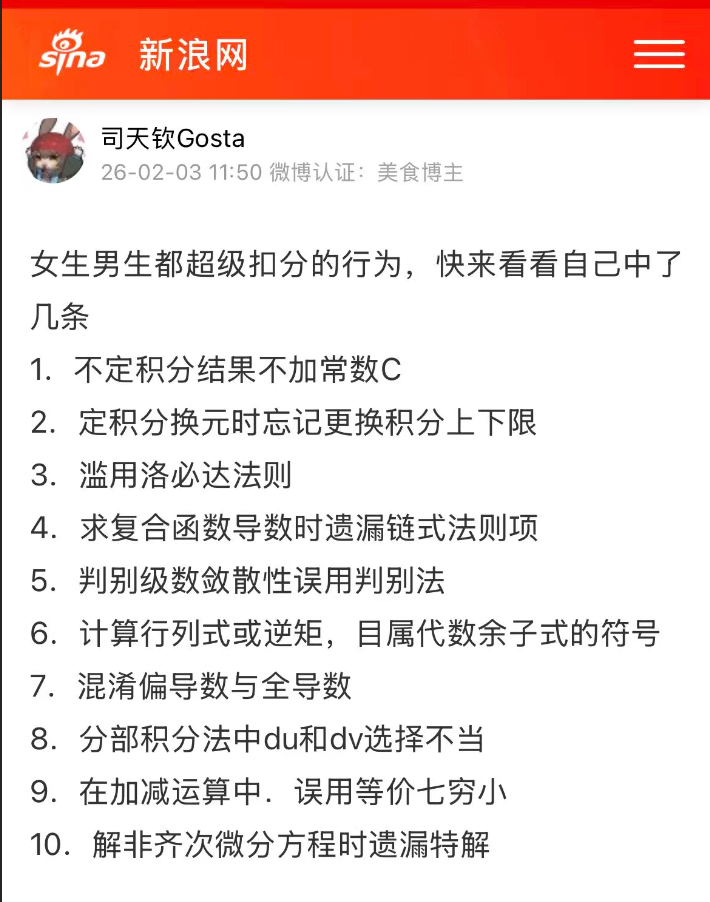
\includegraphics[width=0.38\textwidth]{figures/calculus_turnoffs_meme.png}
  \vfill
\end{frame}

\begin{frame}{Don't mix $d$ and $\partial$}
  \small
  Girlfriend's happiness $H(e,m)=e+2m$: effort $e$ (time, housework)
  and gifts $m$ (a Herm\`es bag).

  \medskip
  After the bag, you need less effort: $e(m)=3-m$, so $e'(m)=-1<0$.

  \medskip
  \textbf{Partial.}\ $\dfrac{\partial H}{\partial m}=2$: more gifts, holding $e$ fixed.

  \medskip
  \textbf{Total.}\ Effort also falls, so
  \[
    \frac{dH}{dm}
    =\frac{\partial H}{\partial e}\,e'(m)+\frac{\partial H}{\partial m}
    =1\cdot(-1)+2=1.
  \]
  The total effect is smaller than the partial: the bag substitutes for time.
\end{frame}

\section{2.1 --- Implicit Function Theorem}

\begin{frame}{2.1 Endogenous vs.\ exogenous --- supply and demand}
  \small
  In a competitive market, demand and supply determine an equilibrium
  \textbf{price} and \textbf{quantity}. Not everything in that picture is
  determined the same way.

  \medskip
  \textbf{Exogenous} (taken as given, from \textbf{outside} the model):
  things that shift the curves --- harvest / weather, costs, income, tastes,
  a tax, population, \ldots\
  Call a typical shifter $\theta$.

  \medskip
  \textbf{Endogenous} (solved for \textbf{inside} the model):
  equilibrium price $p^*$ and quantity $q^*$.
  They adjust until $D=S$.

  \medskip
  {\scriptsize Slopes of $D$ and $S$ are also usually treated as exogenous
  parameters. The model takes them as given and then finds $p^*,q^*$.}
\end{frame}

\begin{frame}{2.1 Example --- eggs in a competitive market}
  \small
  \textbf{Market.}\ Many buyers and many sellers of eggs; take the market
  price as given (competitive). Demand is for eggs as a daily staple.

  \medskip
  \textbf{Exogenous} (shifters, not chosen in this market):
  \begin{itemize}
    \item feed costs, weather / disease on farms (supply)
    \item household income, taste for breakfast, a tax or subsidy (demand or supply)
  \end{itemize}

  \medskip
  \textbf{Endogenous} (solved in this market):
  the egg price $p^*$ and quantity sold $q^*$.

  \medskip
  If feed costs jump (exogenous supply shock), the supply curve shifts.
  Then endogenous $p^*$ and $q^*$ adjust to a new equilibrium.
\end{frame}

\begin{frame}{2.1 Egg market --- a feed-cost shock}
  \begin{center}
    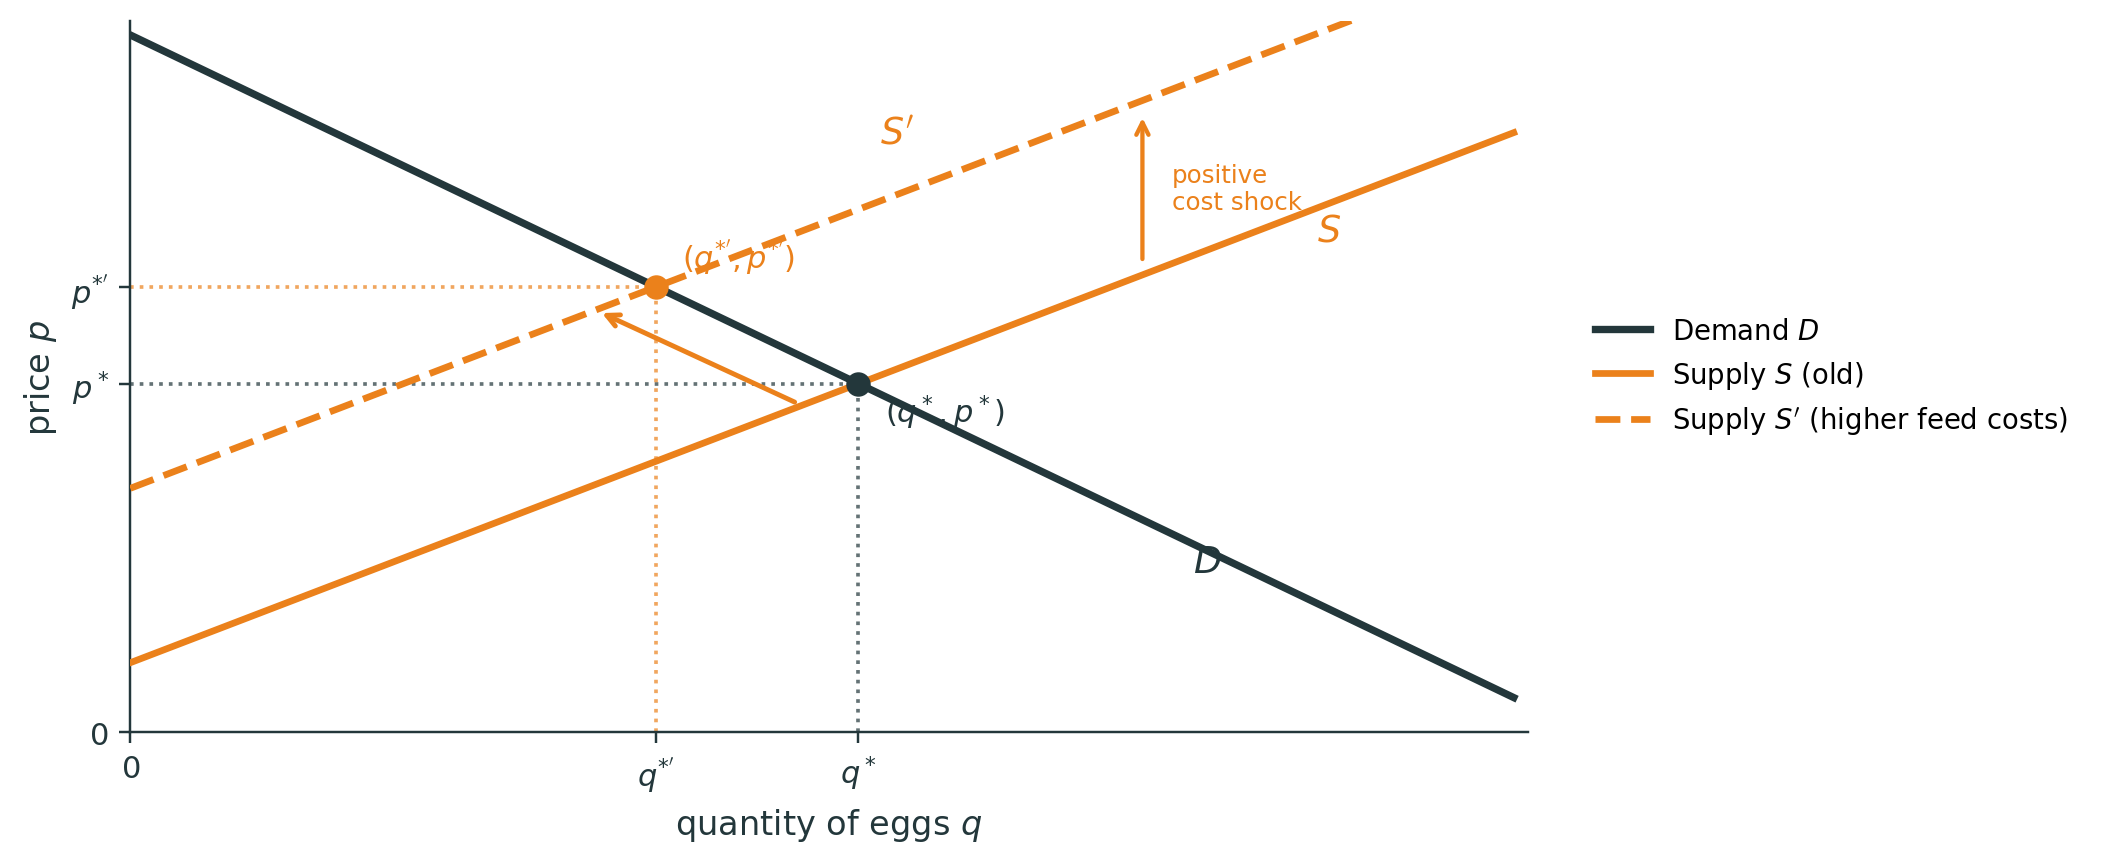
\includegraphics[height=0.62\textheight]{figures/egg_market_supply_shock.png}
  \end{center}
  {\footnotesize Positive cost shock $=$ negative supply shock
  ($S$ left; $p^*$ up, $q^*$ down).}
\end{frame}

\begin{frame}{2.1 Motivation --- comparative statics}
  \small
  Once $p^*$ is determined by exogenous $\theta$, a natural question is:
  if $\theta$ changes, how does the \textbf{endogenous} equilibrium move?

  \medskip
  \textbf{Comparative statics:}\ how $p^*(\theta)$ (and $q^*(\theta)$) respond
  to a shift in an exogenous parameter. We want $\dfrac{dp^*}{d\theta}$.

  \medskip
  \textbf{Eggs.}\ Higher feed costs $\Rightarrow$ supply shifts left
  $\Rightarrow$ $p^*$ typically rises and $q^*$ falls.
  We want a systematic way to get the sign and magnitude.

  \medskip
  Same pattern for a demand shifter (income, tastes), a tax, \ldots\
  The tool is the same once equilibrium is written as $F(p,\theta)=0$.
\end{frame}

\begin{frame}{2.1 Market clearing}
  \small
  Quantity demanded equals quantity supplied:
  \[
    D(p,\theta)=S(p,\theta).
  \]
  Exogenous $\theta$ is a shifter (supply shock, demand shock, tax, \ldots);
  endogenous $p$ and $q$ adjust.

  \medskip
  Excess demand
  \[
    E(p,\theta)=D(p,\theta)-S(p,\theta)
  \]
  is zero at equilibrium: $E(p^*(\theta),\theta)=0$.

  \medskip
  \textbf{Question.}\ How do $p^*$ and $q^*$ change when $\theta$ changes?
\end{frame}

\begin{frame}{2.1 Linear market --- an analytical solution}
  \footnotesize
  Linear demand and supply; supply shifter $s$, demand intercept $\alpha$:
  \[
    D(p,\alpha)=\alpha-bp,
    \qquad
    S(p,s)=s+dp,
    \qquad
    b,d>0.
  \]

  \medskip
  Market clearing $D=S$ gives both endogenous variables in closed form:
  \[
    p^*(s,\alpha)=\frac{\alpha-s}{b+d},
    \qquad
    q^*(s,\alpha)=\alpha-bp^*=\frac{\alpha d+bs}{b+d}.
  \]

  \medskip
  We can differentiate these formulas directly --- no new theorem yet.
\end{frame}

\begin{frame}{2.1 Supply shock vs.\ demand shock}
  \footnotesize
  \textbf{Positive supply shock} ($s\uparrow$; equivalently a negative cost shock):
  \[
    \frac{dp^*}{ds}=-\frac{1}{b+d}<0,
    \qquad
    \frac{dq^*}{ds}=\frac{b}{b+d}>0.
  \]
  Price falls, quantity rises: $p^*$ and $q^*$ move in \textbf{opposite} directions.

  \medskip
  \textbf{Positive demand shock} ($\alpha\uparrow$; income, tastes, \ldots):
  \[
    \frac{dp^*}{d\alpha}=\frac{1}{b+d}>0,
    \qquad
    \frac{dq^*}{d\alpha}=\frac{d}{b+d}>0.
  \]
  Both price and quantity rise: $p^*$ and $q^*$ move in the \textbf{same} direction.
\end{frame}

\begin{frame}{2.1 Supply shock vs.\ demand shock}
  \begin{center}
    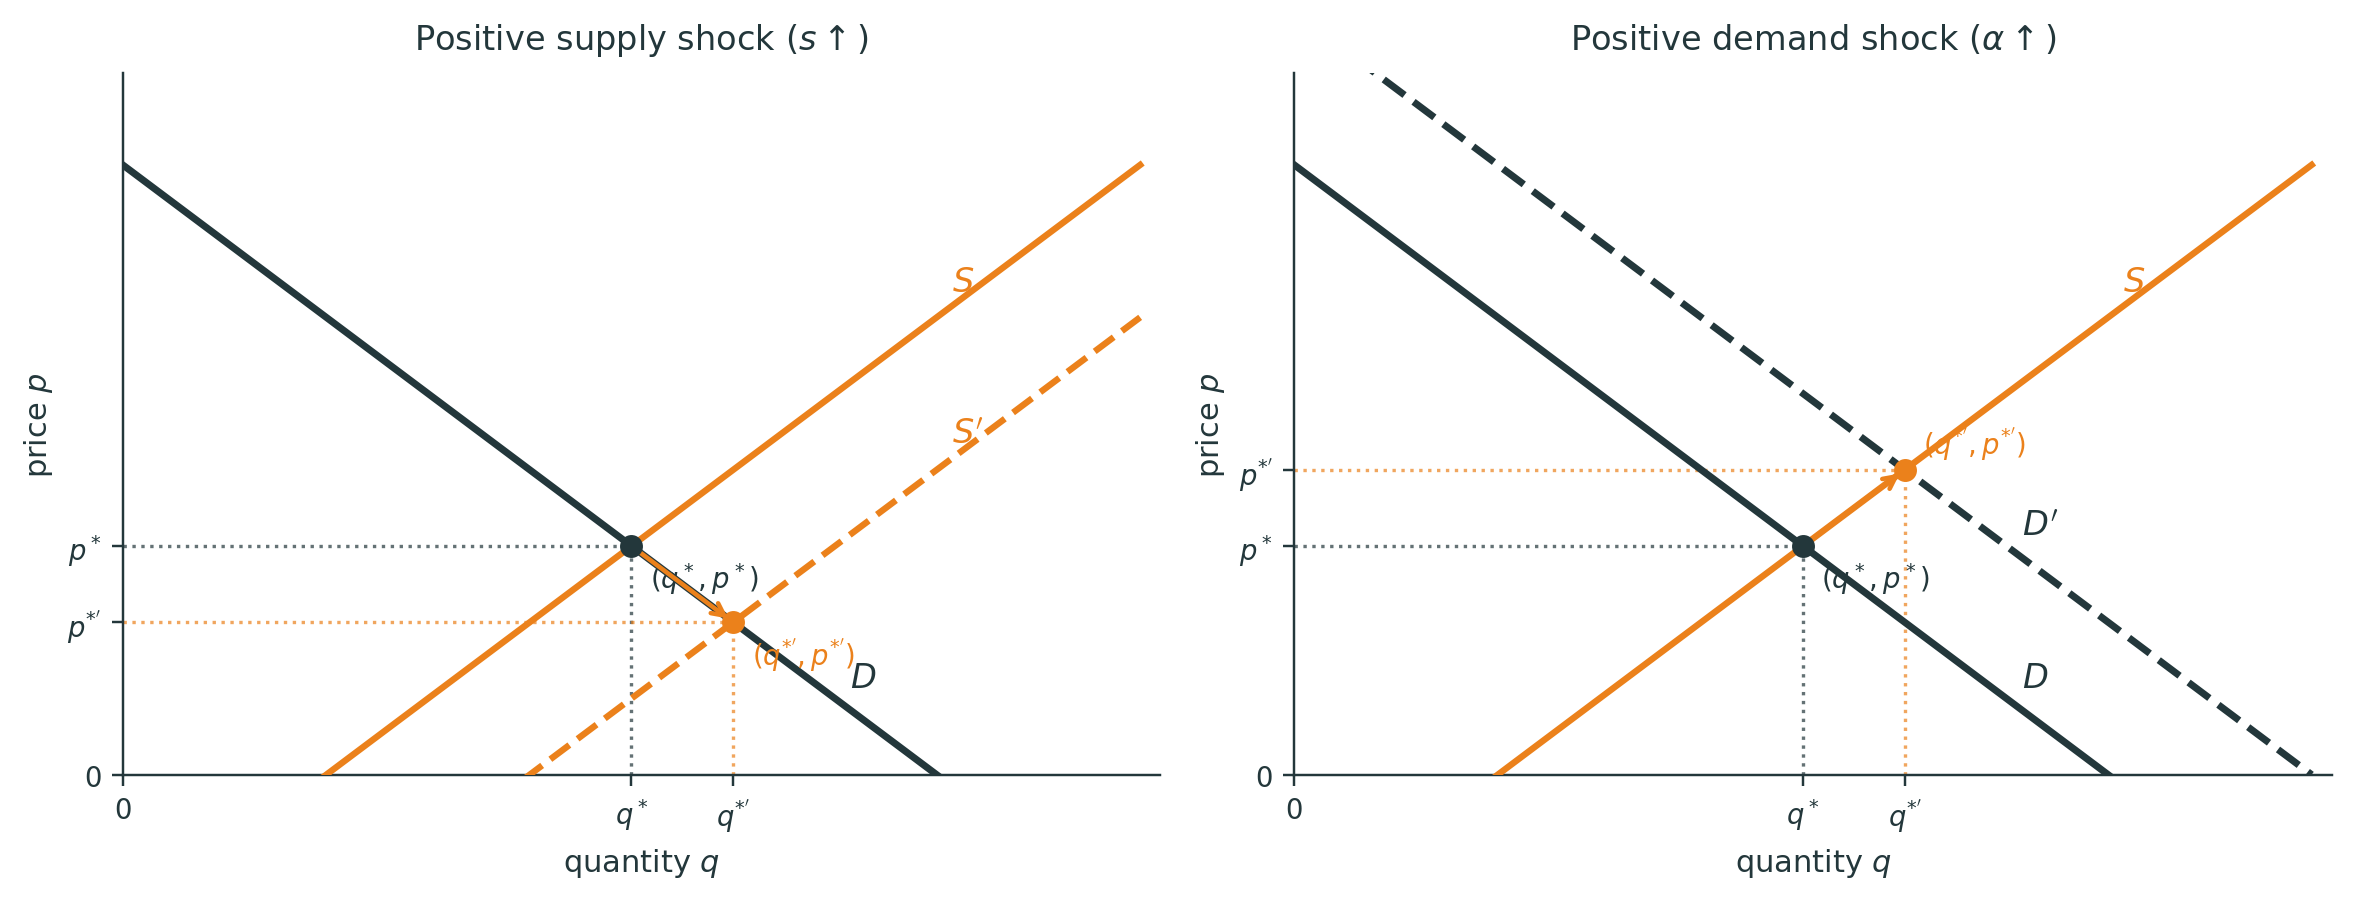
\includegraphics[width=0.98\textwidth]{figures/linear_market_two_shocks.png}
  \end{center}
  {\footnotesize Left: $s\uparrow$ --- $p^*$ down, $q^*$ up.
  Right: $\alpha\uparrow$ --- both $p^*$ and $q^*$ up.}
\end{frame}

\begin{frame}{2.1 Explicit vs.\ implicit}
  \small
  \textbf{Explicit} (what we just did):\ we solved for $p^*$ and $q^*$ as
  formulas in the exogenous variables, e.g.\
  \[
    p^*=g(s,\alpha)=\frac{\alpha-s}{b+d}.
  \]
  Then ordinary differentiation gives $\dfrac{dp^*}{ds}$, $\dfrac{dq^*}{ds}$,
  and the demand-shock derivatives.

  \medskip
  \textbf{Implicit:}\ we only have an equation $F(p,\theta)=0$
  (e.g.\ $E(p,\theta)=0$). We \textbf{know} $F$, but may not be able to write
  $p^*=g(\theta)$ in closed form.

  \medskip
  Next: a nonlinear market where we cannot solve for $p^*$.
\end{frame}

\begin{frame}{2.1 No closed form --- nonlinear market}
  \footnotesize
  Nonlinear demand, with the same two shifters as before:
  \[
    D(p,\alpha)=\alpha e^{-p},
    \qquad
    S(p,s)=s+p,
    \qquad
    \alpha>0,\ s\ge 0.
  \]
  Clearing: $\alpha e^{-p}=s+p$, or $E(p,\alpha,s)=\alpha e^{-p}-s-p=0$.

  \medskip
  This \textbf{defines} $p^*(\alpha,s)$ and $q^*=s+p^*$, but has
  \textbf{no elementary closed form}.
  We cannot write $p^*=g(\alpha,s)$ and differentiate.

  \medskip
  We still want how $p^*$ and $q^*$ respond to a demand shock $\alpha$
  and a supply shock $s$. That is the IFT.
\end{frame}

\begin{frame}{2.1 What problem does the IFT solve?}
  \small
  An equilibrium condition $F(x,\theta)=0$ defines $x^*(\theta)$ \textbf{implicitly}.
  We want $\dfrac{dx^*}{d\theta}$ without solving for $x^*(\theta)$.

  \medskip
  \textbf{IFT:}\ if $F$ is well-behaved and $F_x\neq 0$ at the equilibrium,
  then $x^*(\theta)$ exists locally as a function, and
  \[
    \frac{dx^*}{d\theta}=-\frac{F_\theta}{F_x}
  \]
  --- computed from partials of $F$ only.

  \medskip
  Same idea as the linear market, but it still works when there is no formula
  for $x^*(\theta)$.
\end{frame}

\begin{frame}{2.1 One-variable IFT --- statement}
  \footnotesize
  Let $F(x,y)$ be $C^1$ near $(x_0,y_0)$ with $F(x_0,y_0)=0$.
  If $F_y(x_0,y_0)\neq 0$, then locally there is a unique $g$ such that
  \[
    y=g(x),
    \qquad
    F(x,g(x))=0,
    \qquad
    g(x_0)=y_0,
  \]
  and
  \[
    \boxed{
      g'(x)=-\frac{F_x(x,y)}{F_y(x,y)}
    }
    \qquad\text{on the curve }F(x,y)=0.
  \]

  \medskip
  {\scriptsize Several variables (\InterestOnly):
  \AppendixLink{sec:ift-multivar}.}
\end{frame}

\begin{frame}{2.1 Why $F_y \neq 0$? --- regularity condition}
  \small
  \textbf{Left:}\ $F_y \neq 0$ at $(x_0,y_0)$ --- tangent has finite slope;
  locally $y=g(x)$.
  \hfill
  \textbf{Right:}\ $F_y=0$ at $(0,0)$ --- \textbf{vertical tangent};
  $\dfrac{dy}{dx}=-F_x/F_y$ is undefined.

  \medskip
  \centering
  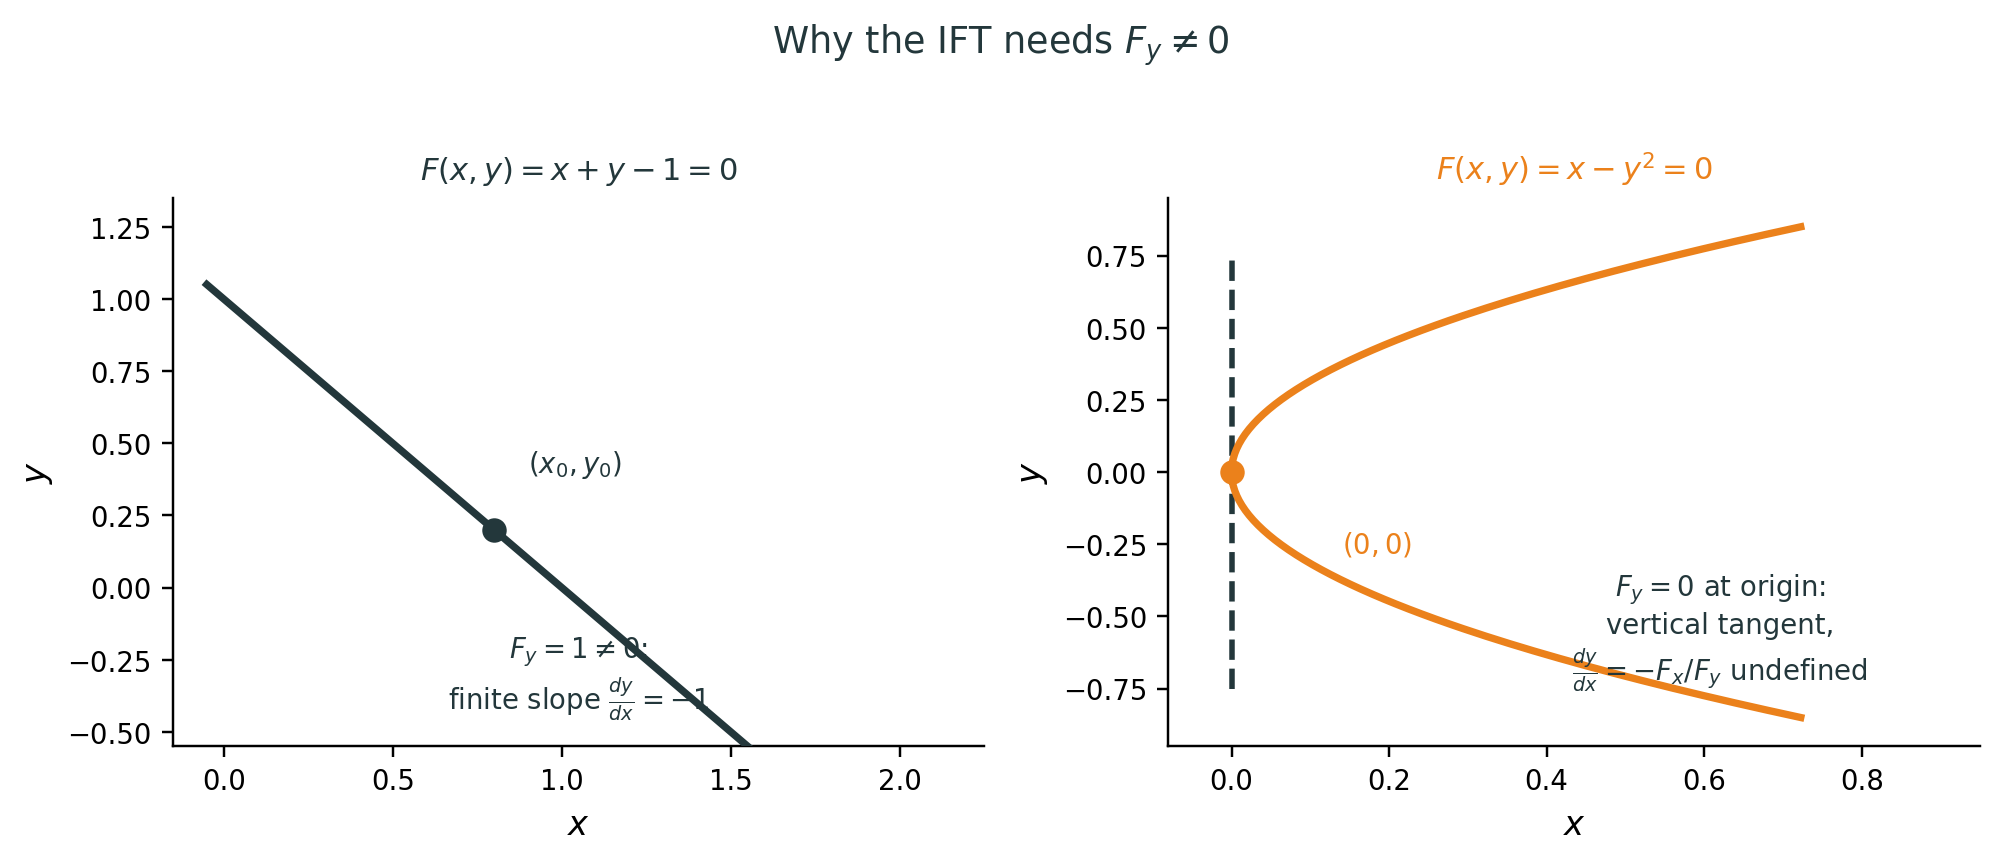
\includegraphics[width=0.92\textwidth]{figures/ift_regularity_condition.png}

  \medskip
  {\footnotesize Near $(0,0)$ on $x=y^2$, the curve is vertical in the $(x,y)$-plane,
  so $y$ cannot be written as a single-valued function of $x$.}
\end{frame}

\begin{frame}{2.1 Check --- IFT recovers the linear answer}
  \footnotesize
  Return to $E(p,s)=\alpha-s-(b+d)p$.
  Partials: $E_p=-(b+d)\neq 0$,\ $E_s=-1$.

  \medskip
  \textbf{IFT:}
  \[
    \frac{dp^*}{ds}=-\frac{E_s}{E_p}=-\frac{-1}{-(b+d)}=-\frac{1}{b+d}<0.
  \]
  Same as differentiating $p^*(s)=(\alpha-s)/(b+d)$ explicitly.

  \medskip
  \textbf{Interpretation (direct vs.\ indirect).}\
  Higher $s$ lowers excess demand at the old price ($E_s<0$: surplus).
  Price must fall ($E_p<0$) until $E=0$ is restored.
\end{frame}

\begin{frame}{2.1 Nonlinear market --- two shocks}
  \footnotesize
  Same market:
  \[
    D(p,\alpha)=\alpha e^{-p},
    \qquad
    S(p,s)=s+p,
    \qquad
    E(p,\alpha,s)=\alpha e^{-p}-s-p=0.
  \]
  IFT, with $q^*=s+p^*$. Same signs as the linear market.

  \medskip
  \textbf{Demand shock} $\alpha\uparrow$:
  \[
    \frac{dp^*}{d\alpha}=\frac{e^{-p^*}}{\alpha e^{-p^*}+1}>0,
    \qquad
    \frac{dq^*}{d\alpha}=\frac{dp^*}{d\alpha}>0.
  \]

  \medskip
  \textbf{Supply shock} $s\uparrow$:
  \[
    \frac{dp^*}{ds}=-\frac{1}{\alpha e^{-p^*}+1}<0,
    \qquad
    \frac{dq^*}{ds}=\frac{\alpha e^{-p^*}}{\alpha e^{-p^*}+1}>0.
  \]
\end{frame}

\begin{frame}{2.1 Nonlinear market --- two shocks}
  \begin{center}
    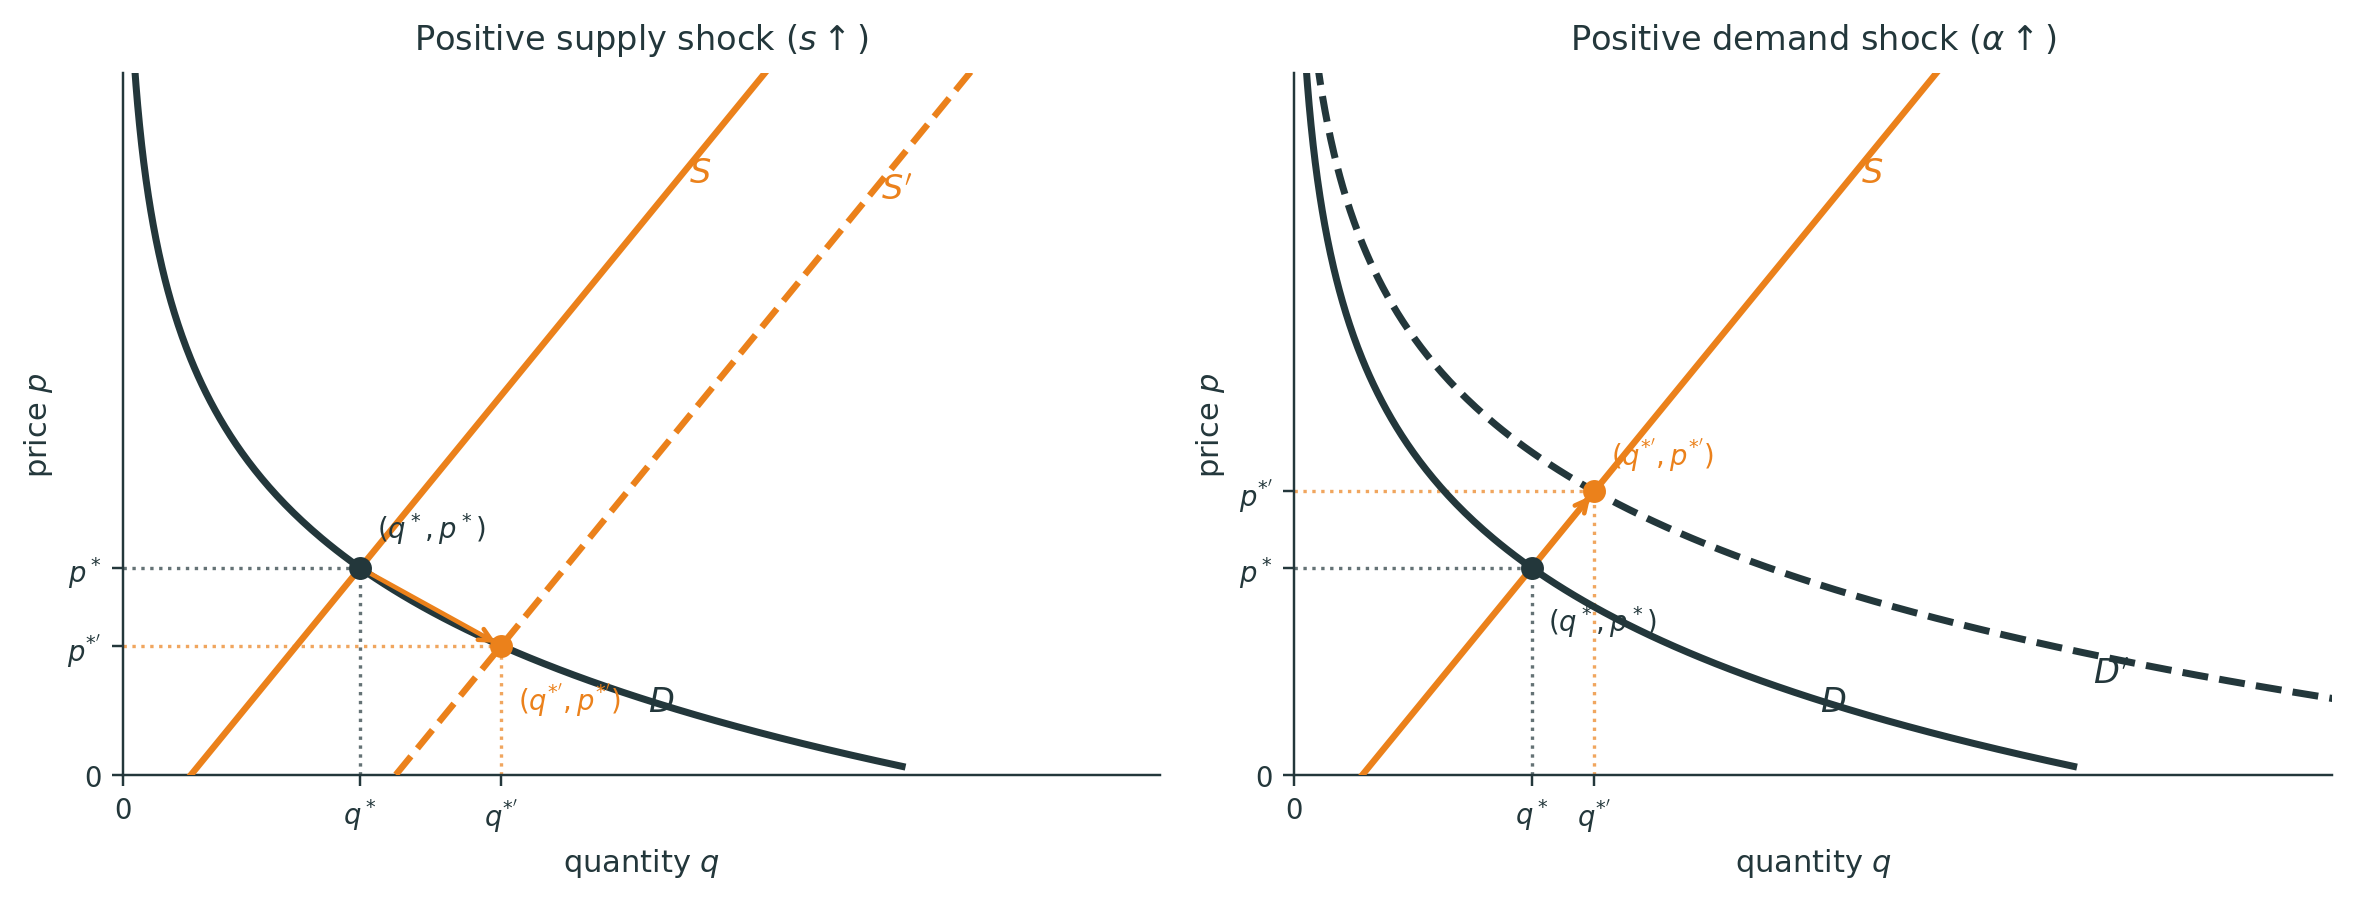
\includegraphics[width=0.98\textwidth]{figures/nonlinear_market_two_shocks.png}
  \end{center}
  {\footnotesize Left: $s\uparrow$ --- $p^*$ down, $q^*$ up.
  Right: $\alpha\uparrow$ --- both $p^*$ and $q^*$ up.}
\end{frame}

\begin{frame}{2.1 Tax incidence --- competitive passthrough}
  \footnotesize
  Perfect competition. Unit tax $t$ on sellers: buyers pay $p$, sellers receive $p-t$.
  \[
    E(p,t)=D(p)-S(p-t)=0.
  \]
  IFT: $E_p=D'-S'$, $E_t=S'$, so
  \[
    \frac{dp}{dt}=-\frac{E_t}{E_p}=\frac{S'}{S'-D'}\in(0,1),
    \qquad
    \frac{d(p-t)}{dt}=\frac{D'}{S'-D'}\in(-1,0).
  \]
  With $\varepsilon_D=D'(p)\,p/q<0$ and $\varepsilon_S=S'(p)\,p/q>0$,
  \[
    \frac{dp}{dt}=\frac{\varepsilon_S}{\varepsilon_S+|\varepsilon_D|}.
  \]
  The \textbf{less elastic} side bears more of the tax
  (inelastic demand $\Rightarrow$ buyers; inelastic supply $\Rightarrow$ sellers).
\end{frame}

\section{2.2 --- EVT, MVT, and Existence}

\begin{frame}{2.2 EVT on a closed interval $[a,b]$}
  \footnotesize
  \textbf{Extreme Value Theorem (EVT).}\
  If $f$ is \textbf{continuous} on the \textbf{closed} interval $[a,b]$, then $f$ attains a
  \textbf{maximum} and a \textbf{minimum} on $[a,b]$.

  \medskip
  So $\exists\,c,d\in[a,b]$ such that
  \[
    f(c)\le f(x)\le f(d)
    \qquad\text{for all } x\in[a,b].
  \]

  \medskip
  {\scriptsize $[a,b]$ is \textbf{closed and bounded} --- a compact set in $\mathbb{R}$.}
\end{frame}

\begin{frame}[plain]{2.2 When EVT fails}
  \centering
  \vfill
  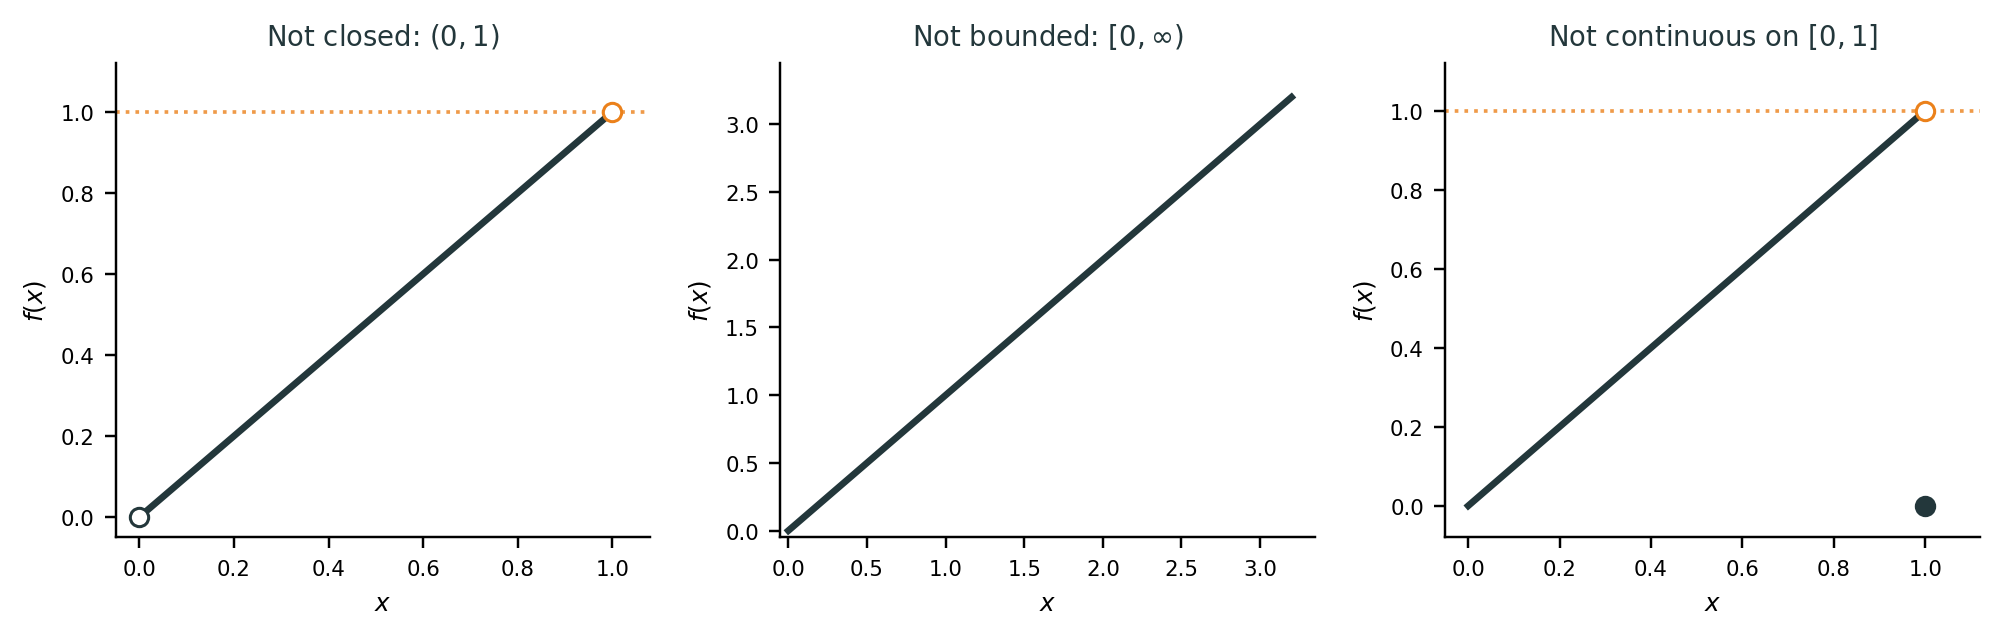
\includegraphics[width=0.96\textwidth]{figures/evt_failures.png}
  \vfill
  {\footnotesize Need continuity on a \textbf{closed, bounded} domain (or compact set more generally).}
\end{frame}

\begin{frame}{2.2 Open and closed sets}
  \footnotesize
  \textbf{Open set} (intuition): every point has a small neighborhood still inside the set.

  \medskip
  \textbf{Closed set} (intuition): contains its \textbf{boundary}; limits of sequences in the set stay in the set.

  \medskip
  \textbf{Economic examples.}
  \begin{itemize}
    \item Budget $\{\mathbf{x}:\mathbf{p}\cdot\mathbf{x}\le B\}$ --- \textbf{closed} (includes the budget line).
    \item Strict budget $\mathbf{p}\cdot\mathbf{x}<B$ --- \textbf{not closed} (boundary excluded).
    \item Reservation price set $P=\{p:p<\bar p\}$ --- not closed; $\sup P=\bar p$ may not be attained.
  \end{itemize}

  \medskip
  {\scriptsize On $\mathbb{R}^1$: $[a,b]$ is closed and bounded; $(a,b)$ is open (not closed).
  The failure figure above: not closed, not bounded, or not continuous.}
\end{frame}

\begin{frame}{2.2 Compact sets and Weierstrass EVT}
  \footnotesize
  \textbf{In $\mathbb{R}^n$ (camp level):}\ a set is \textbf{compact} when it is
  \textbf{closed and bounded} (Heine--Borel, stated).

  \medskip
  \textbf{Weierstrass Extreme Value Theorem.}\
  If $f$ is continuous on a compact set $K\subset\mathbb{R}^n$, then $f$ attains a
  \textbf{maximum} and \textbf{minimum} on $K$.

  \medskip
  \textbf{Why economists care.}\
  \[
    \text{compact feasible set }K
    \;+\;
    \text{continuous objective }f
    \;\Rightarrow\;
    \text{optimum \textbf{exists}}
  \]
  (preview of Day~4 optimization).

  \medskip
  {\scriptsize Proof:
  \AppendixLink{sec:weierstrass-proof} (\InterestOnly).}
\end{frame}

\begin{frame}{2.2 Example --- existence of a utility maximizer}
  \footnotesize
  \textbf{Setup (consumer problem).}\
  Prices $p_1,p_2>0$, income $w>0$, budget set
  \[
    \mathcal{B}
    = \bigl\{(x_1,x_2)\in\mathbb{R}^2_+ : p_1 x_1 + p_2 x_2 \le w\bigr\}.
  \]

  \medskip
  \textbf{1.}\ $\mathcal{B}$ is \textbf{closed} (weak inequality $\le$) and \textbf{bounded}
  (e.g.\ $0\le x_i\le w/p_i$), hence \textbf{compact} in $\mathbb{R}^2$.

  \medskip
  \textbf{2.}\ Suppose utility $u(x_1,x_2)$ is \textbf{continuous} on $\mathcal{B}$.

  \medskip
  \textbf{3.}\ By Weierstrass EVT, $u$ attains a \textbf{maximum} on $\mathcal{B}$.

  \medskip
  \textbf{Conclusion.}\
  An optimal consumption bundle $x^*\in\mathcal{B}$ \textbf{exists}
  (existence theorem for the consumer problem; first-order conditions come on Day~4).

  \medskip
  {\scriptsize \textbf{Not uniqueness.}\
  Weierstrass gives at least one maximizer, not a unique one
  (e.g.\ $u(x_1,x_2)=x_1+x_2$ has many optima on $\mathcal{B}$).
  Uniqueness needs extra conditions (e.g.\ strictly concave / strictly quasiconcave $u$; Day~4).}
\end{frame}

\begin{frame}{2.2 Intermediate Value Theorem}
  \footnotesize
  \begin{columns}[T,onlytextwidth]
    \column{0.52\textwidth}
    \textbf{Intermediate Value Theorem (IVT).}\
    If $f$ is continuous on $[a,b]$ and $k$ lies between $f(a)$ and $f(b)$,
    then $\exists\,c\in[a,b]$ with $f(c)=k$.

    \medskip
    \textbf{Sign-change case.}\
    If $f(a)$ and $f(b)$ have opposite signs, then $\exists\,c\in(a,b)$ with
    $f(c)=0$.

    \medskip
    Continuity is essential: a jump can skip the target value.

    \column{0.44\textwidth}
    \centering
    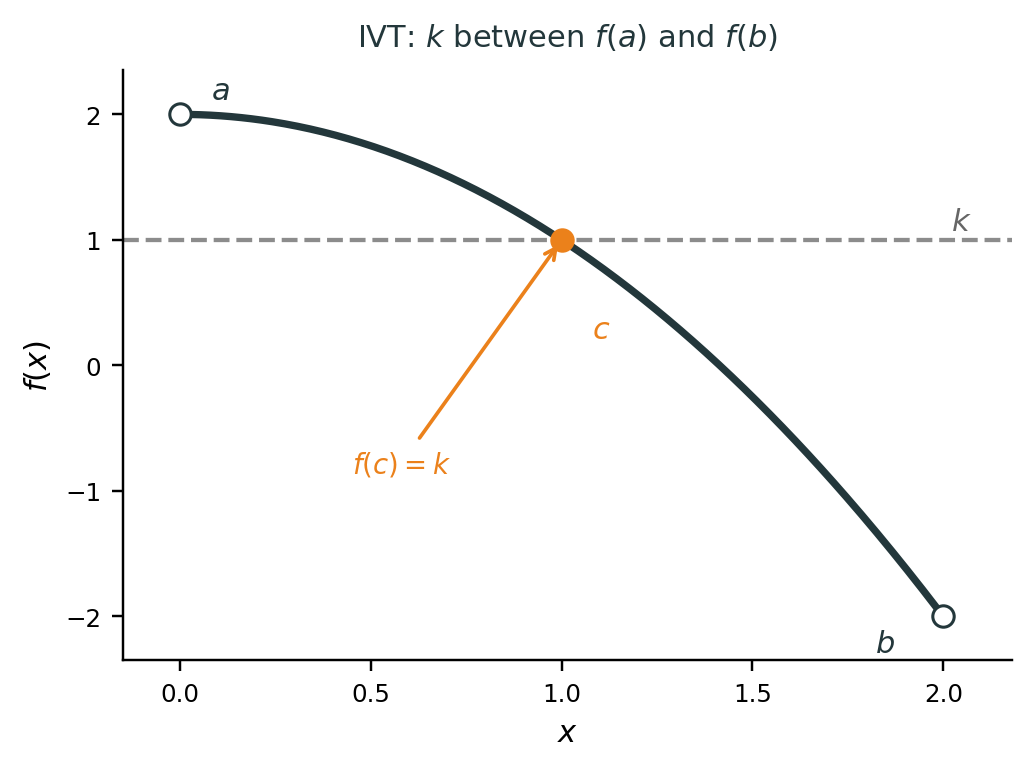
\includegraphics[width=\linewidth]{figures/ivt_generic.png}
  \end{columns}
\end{frame}

\begin{frame}{2.2 Existence of a clearing price}
  \scriptsize
  Same nonlinear market, with numbers plugged in:
  $D(p)=6e^{-p}$, $S(p)=\tfrac12+p$
  (no closed form for $p^*$).
  Excess demand $E(p)=6e^{-p}-\tfrac12-p$ is continuous.
  $E(0)=\tfrac{11}{2}>0$ (shortage) and $E(5)=6e^{-5}-\tfrac{11}{2}<0$ (surplus).
  IVT: $\exists\,p^*\in(0,5)$ with $E(p^*)=0$.
  Also $E'(p)=-6e^{-p}-1<0$, so the root is unique.

  \vspace{2pt}
  \begin{center}
    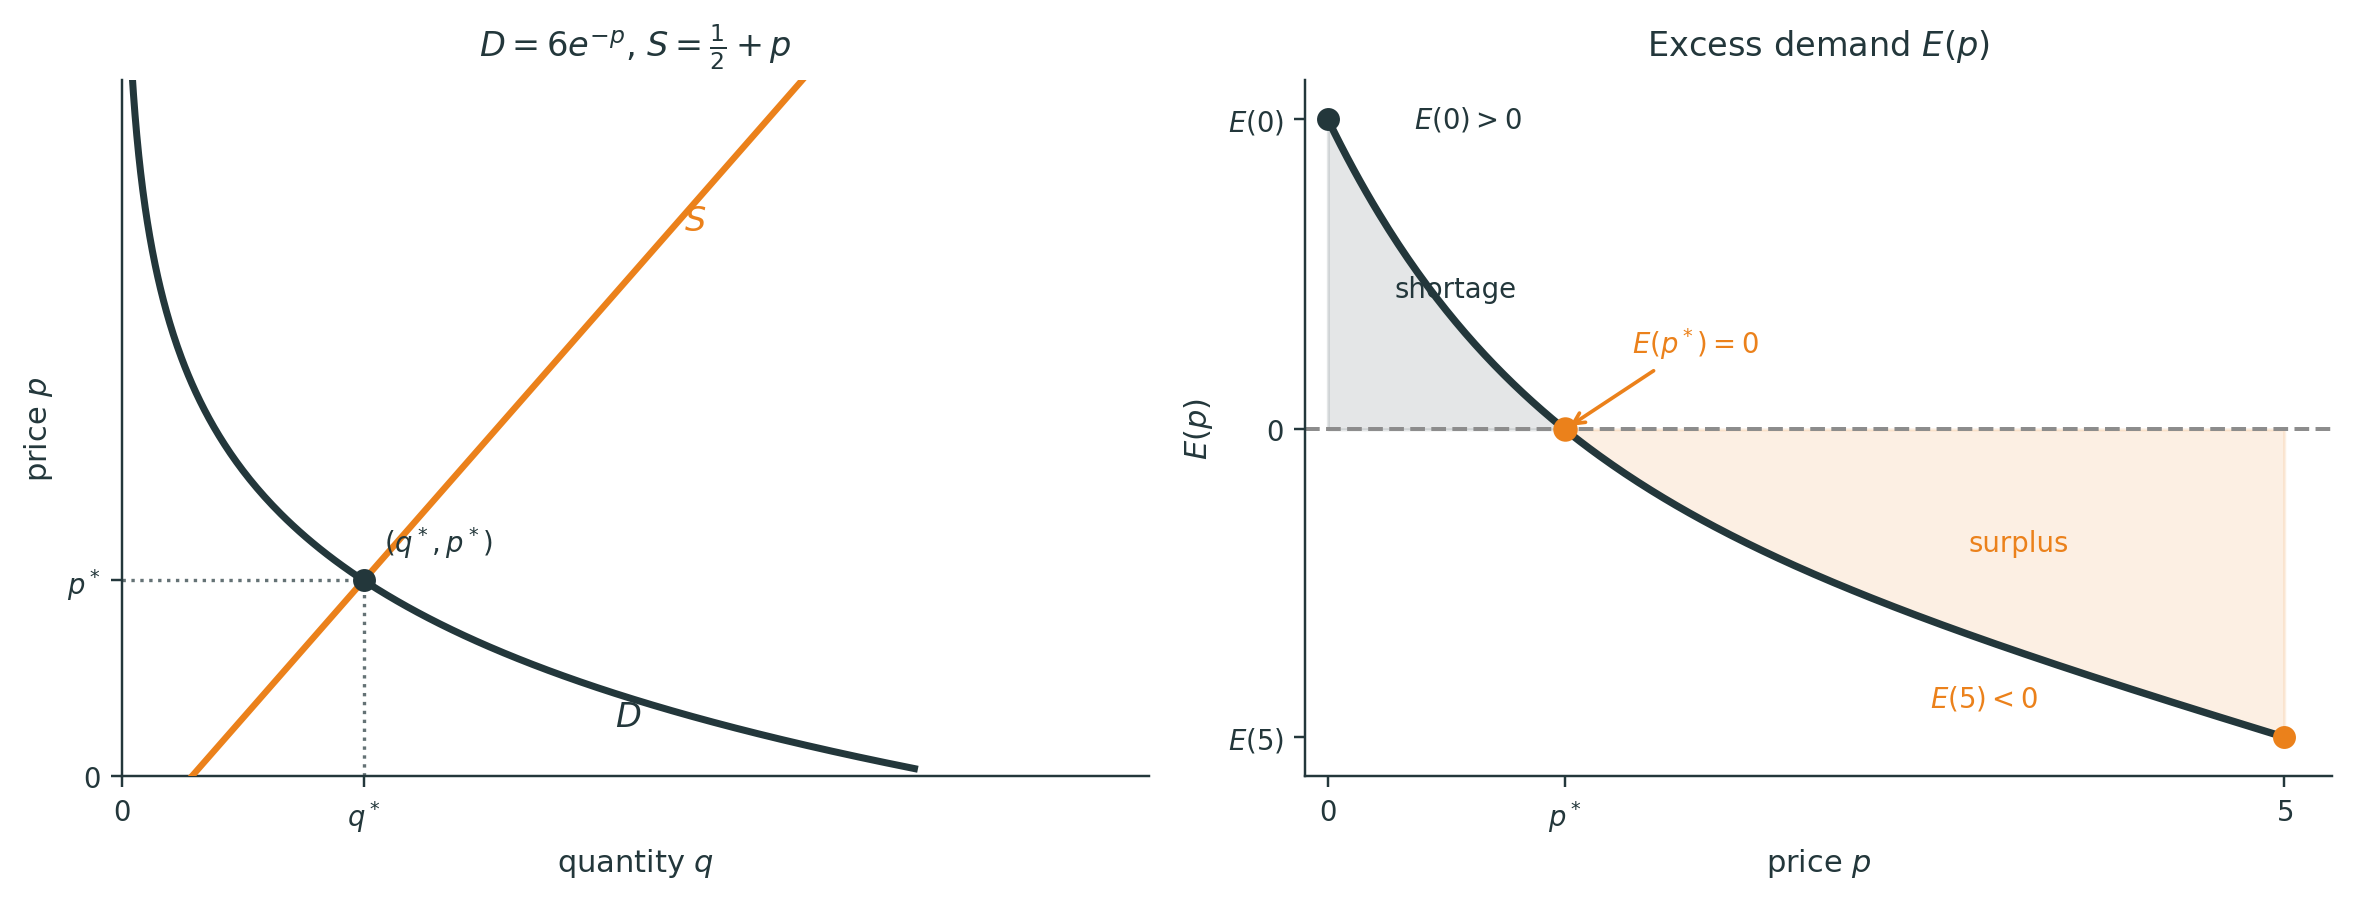
\includegraphics[height=0.52\textheight]{figures/ivt_excess_demand.png}
  \end{center}
\end{frame}

\begin{frame}{2.2 Rolle's theorem}
  \footnotesize
  \begin{columns}[T,onlytextwidth]
    \column{0.52\textwidth}
    \textbf{Rolle's theorem.}\
    If $f$ is continuous on $[a,b]$, differentiable on $(a,b)$, and
    $f(a)=f(b)$, then $\exists\,c\in(a,b)$ with $f'(c)=0$.

    \medskip
    \InterestOnly

    \medskip
    \textbf{Proof.}\
    If $f$ is constant on $[a,b]$, any $c\in(a,b)$ works.
    Otherwise, by EVT, $f$ has a maximum or minimum on $[a,b]$.
    Since $f(a)=f(b)$, this extremum occurs at some \textbf{interior} point
    $c\in(a,b)$.
    At an interior peak or trough, the tangent is horizontal, so $f'(c)=0$.
    \hfill$\square$

    \medskip
    {\scriptsize Special case of the MVT below with $f(a)=f(b)$.}

    \column{0.44\textwidth}
    \centering
    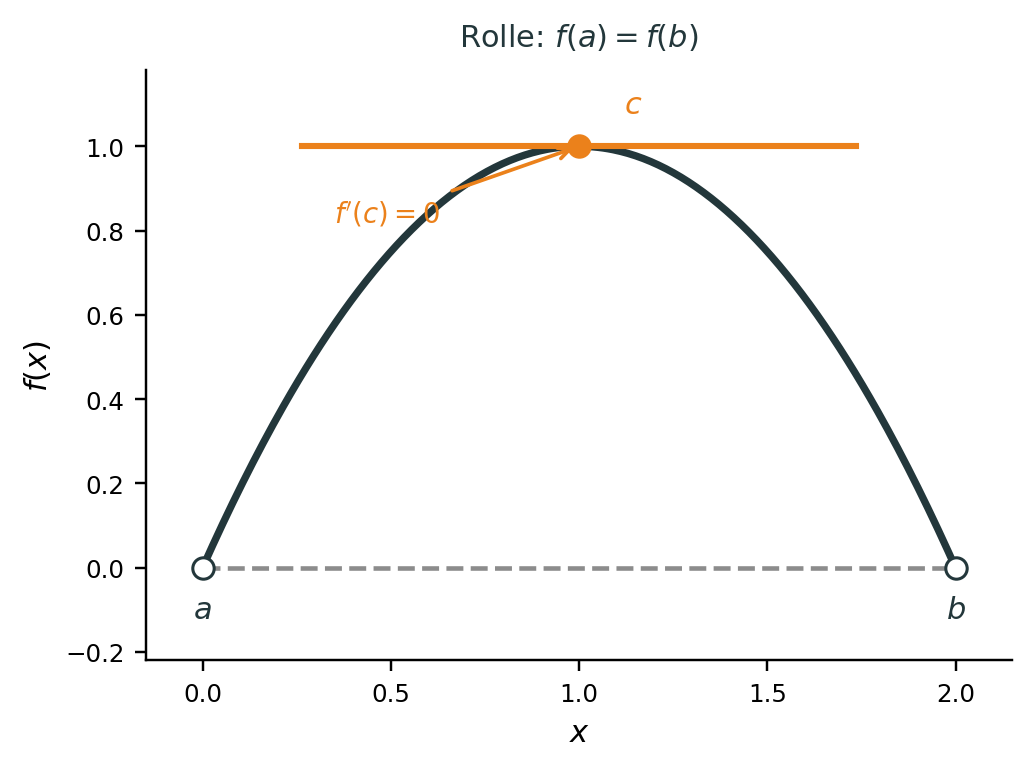
\includegraphics[width=\linewidth]{figures/mvt_rolle.png}
  \end{columns}
\end{frame}

\begin{frame}{2.2 Mean Value Theorem}
  \footnotesize
  \begin{columns}[T,onlytextwidth]
    \column{0.52\textwidth}
    \textbf{Mean Value Theorem (MVT).}\
    If $f$ is continuous on $[a,b]$ and differentiable on $(a,b)$, then
    $\exists\,c\in(a,b)$ such that
    \[
      f'(c)=\frac{f(b)-f(a)}{b-a}.
    \]

    \medskip
    \textbf{Picture:}\ some interior tangent is \textbf{parallel} to the secant
    through $(a,f(a))$ and $(b,f(b))$.

    \medskip
    \textbf{Example.}\ $f(x)=x^2$ on $[0,2]$: secant slope $=2$, so $f'(c)=2c=2$
    gives $c=1$.

    \medskip
    \InterestOnly

    \medskip
    \textbf{Proof idea:}\ define $g(x)=f(x)-m(x-a)$ with
    $m=\dfrac{f(b)-f(a)}{b-a}$; then $g(a)=g(b)$, Rolle gives $f'(c)=m$.

    \column{0.44\textwidth}
    \centering
    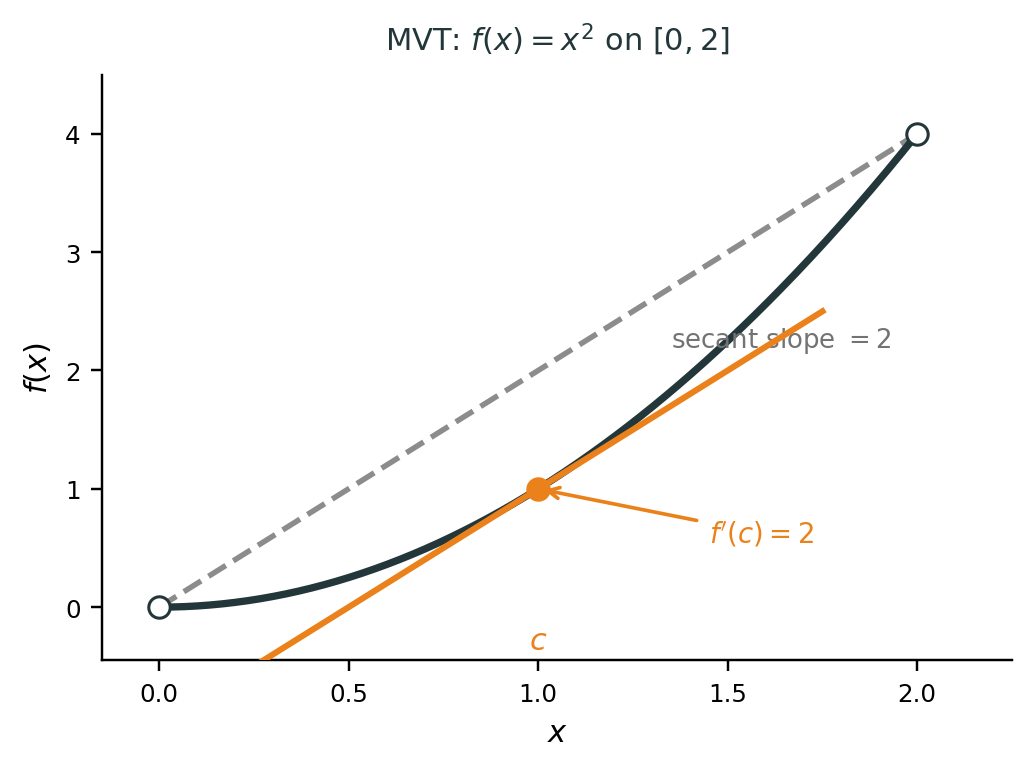
\includegraphics[width=\linewidth]{figures/mvt_secant_tangent.png}
  \end{columns}
\end{frame}

\begin{frame}{2.2 Example --- labor and output (economics)}
  \footnotesize
  \textbf{Setup.}\ Output $f(L)$ from labor $L$; $f$ continuous on $[L_1,L_2]$, differentiable on $(L_1,L_2)$.

  \medskip
  \textbf{MVT.}\ $\exists\,L^*\in(L_1,L_2)$ with
  \[
    f'(L^*)
    = \underbrace{\frac{f(L_2)-f(L_1)}{L_2-L_1}}_{\text{average product gain over }[L_1,L_2]}.
  \]
  At some interior employment level, \textbf{marginal product} $=$ \textbf{average product} of the change.
\end{frame}

\begin{frame}{2.2 MC and AC --- what the crossover means}
  \footnotesize
  \textbf{Cost example.}\ $C(q)=q^2+4$ (fixed cost $4$, rising marginal cost).

  \medskip
  \[
    \mathrm{MC}(q)=C'(q)=2q,
    \qquad
    \mathrm{AC}(q)=\frac{C(q)}{q}=q+\frac{4}{q}.
  \]

  \medskip
  \textbf{MVT link.}\ On $[0,\bar q]$, $\exists\,q^*\in(0,\bar q)$ with
  $\mathrm{MC}(q^*)=\dfrac{C(\bar q)-C(0)}{\bar q}=\bar q$:
  marginal cost somewhere equals the \textbf{average incremental cost} of the first $\bar q$ units.
  (If $C(0)=0$, this is $\mathrm{AC}(\bar q)$.)

  \medskip
  \textbf{Why MC crosses AC at the minimum of AC.}\
  Minimizing $\mathrm{AC}(q)=C(q)/q$ gives $\mathrm{MC}(q)=C(q)/q$ (FOC) $\Rightarrow$ curves cross at $q^*=2$.
  \begin{itemize}
    \item For $q<q^*$: $\mathrm{MC}<\mathrm{AC}$ $\Rightarrow$ an extra unit pulls the average \textbf{down}.
    \item For $q>q^*$: $\mathrm{MC}>\mathrm{AC}$ $\Rightarrow$ an extra unit pulls the average \textbf{up}.
    \item At $q^*$: the last unit costs exactly the average --- \textbf{efficient scale} (lowest cost per unit).
  \end{itemize}
\end{frame}

\begin{frame}[plain]{2.2 MC and AC --- graph}
  \centering
  \vfill
  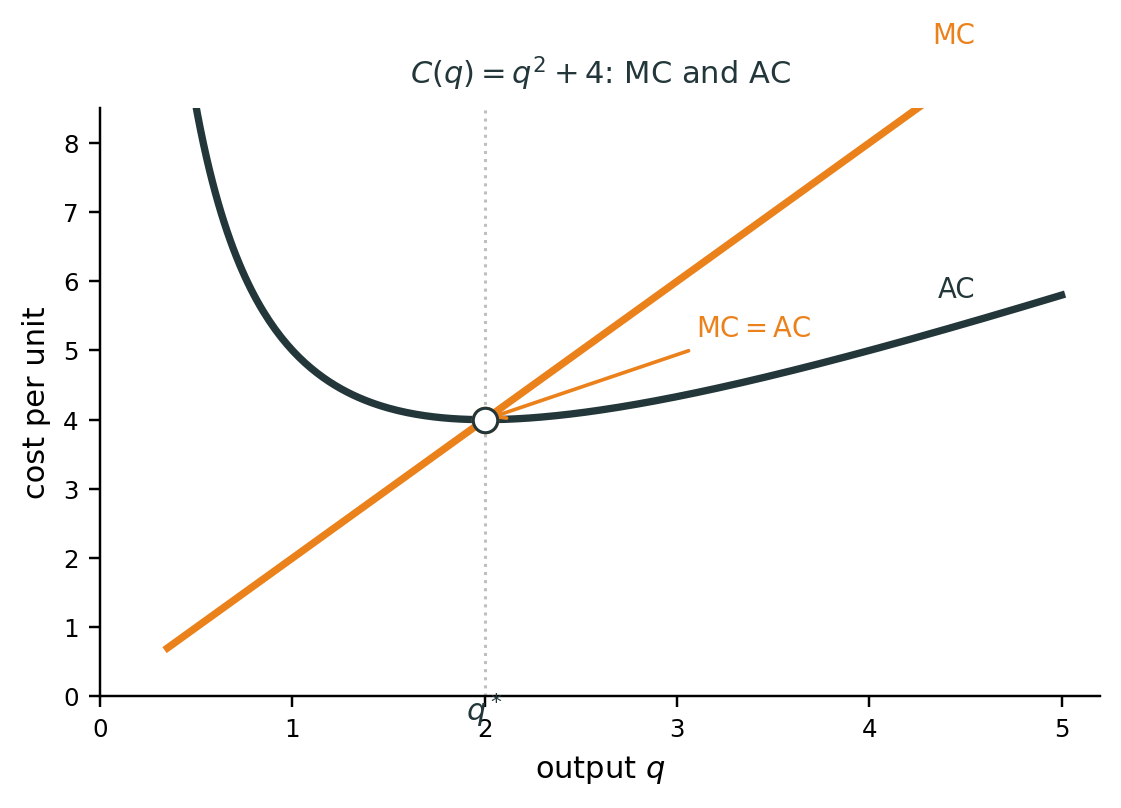
\includegraphics[width=0.72\textwidth]{figures/mvt_mc_ac.png}
  \vfill
\end{frame}

\section{2.3 --- Integration and Probability}

\begin{frame}{2.3 Integral as area and accumulation}
  \footnotesize
  \begin{columns}[T,onlytextwidth]
    \column{0.48\textwidth}
    \textbf{Riemann idea.}\ For $f\ge 0$ on $[a,b]$,
    \[
      \int_a^b f(x)\,dx
      \approx \sum_{i=1}^n f(x_i^*)\,\Delta x
    \]
    is the \textbf{signed area} under the curve / total accumulation.

    \medskip
    \textbf{Definite vs indefinite.}
    \begin{itemize}
      \item Definite: $\displaystyle\int_a^b f(x)\,dx$ is a number
      \item Indefinite: $\displaystyle\int f(x)\,dx=F(x)+C$ is a family of antiderivatives
    \end{itemize}

    \medskip
    {\scriptsize Econ: total cost, consumer surplus, probability mass.}

    \column{0.50\textwidth}
    \centering
    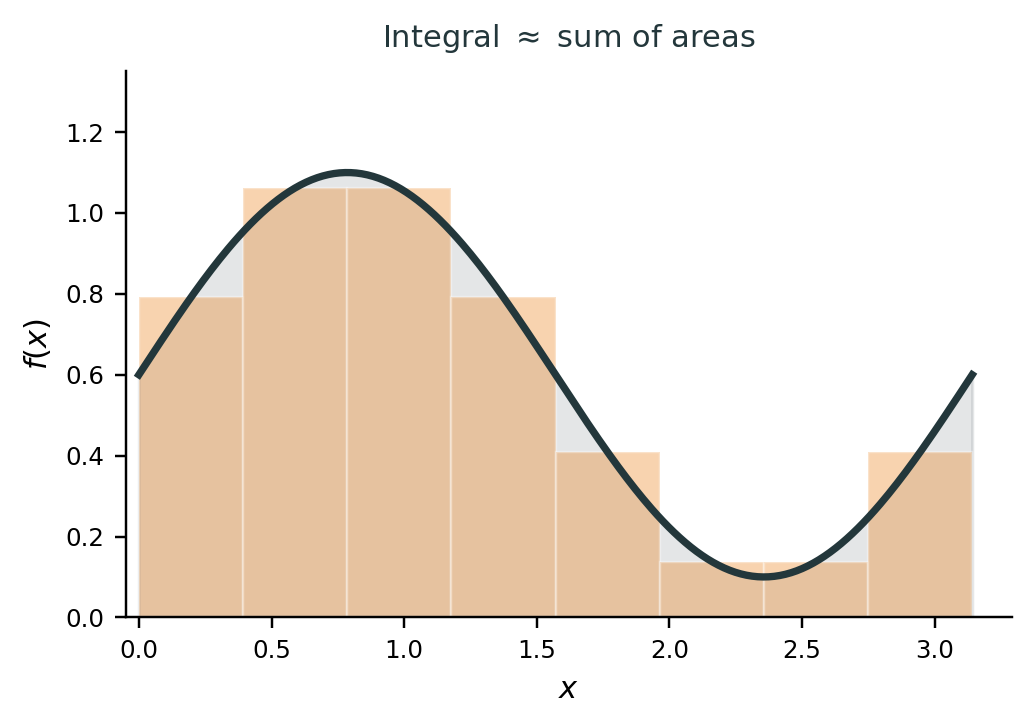
\includegraphics[width=\linewidth]{figures/riemann_area.png}
  \end{columns}
\end{frame}

\begin{frame}{2.3 Riemann vs.\ Lebesgue --- for interest}
  \footnotesize
  \textcolor{mAccent}{\textbf{Not required for Math Camp.}}

  \medskip
  \textbf{Two ways to define $\displaystyle\int f$.}

  \medskip
  \begin{tabular}{@{}p{0.46\textwidth}p{0.46\textwidth}@{}}
    \textbf{Riemann (this camp)} &
    \textbf{Lebesgue (grad / probability)} \\
    \midrule
    Chop the \textbf{$x$-axis} into small pieces &
    Chop the \textbf{$y$-axis} into levels \\
    Sum (height) $\times$ (width) &
    Sum (level) $\times$ (measure of set where $f$ hits that level) \\
    Good for hand calculations &
    Integrates more pathological functions \\
    Area under curve picture &
    Foundation for modern probability \\
  \end{tabular}

  \medskip
  \textbf{Contrast in one sentence.}\
  Riemann slices \textbf{vertically}; Lebesgue slices \textbf{horizontally} by value.
\end{frame}

\begin{frame}{2.3 Lebesgue integral --- for interest}
  \footnotesize
  \textcolor{mAccent}{\textbf{Not required for Math Camp.}}

  \medskip
  \textbf{When Riemann fails.}\
  Riemann needs the function to be ``well behaved'' on intervals:
  too many jumps can prevent upper and lower sums from converging to the same number.

  \medskip
  \textbf{Classic example (not Riemann integrable).}\
  Dirichlet function on $[0,1]$:
  \[
    f(x)=
    \begin{cases}
      1, & x\in\mathbb{Q},\\
      0, & x\notin\mathbb{Q}.
    \end{cases}
  \]
  Every interval contains rationals and irrationals, so upper and lower Riemann sums
  never agree --- no Riemann integral.

  \medskip
  \textbf{Lebesgue handles this.}\
  It integrates by \textbf{level sets}, so a ``sparse'' jump set like $\mathbb{Q}$ does
  not block integration the way Riemann's interval partitions do.
\end{frame}

\begin{frame}{2.3 Fundamental Theorem of Calculus}
  \footnotesize
  \textbf{Part I.}\ If $F'(x)=f(x)$, then
  \[
    \int_a^b f(x)\,dx = F(b)-F(a).
  \]

  \medskip
  \textbf{Part II.}\ If $f$ is continuous and $F(x)=\displaystyle\int_a^x f(t)\,dt$, then
  $F'(x)=f(x)$.

  \medskip
  {\scriptsize Differentiation and integration are inverse operations (MVT underlies many proofs).}
\end{frame}

\begin{frame}{2.3 Integration by parts}
  \footnotesize
  \textbf{From the product rule.}\
  For differentiable $u(x)$ and $v(x)$,
  \[
    (uv)' = u'v + uv'
    \quad\Rightarrow\quad
    uv' = (uv)' - u'v.
  \]
  Integrate both sides:
  \[
    \int u\,v'\,dx = uv - \int u'v\,dx
    \qquad\text{or}\qquad
    \boxed{\int u\,dv = uv - \int v\,du}.
  \]

  \medskip
  On $[a,b]$ with $u'v$ integrable,
  \[
    \int_a^b u(x)v'(x)\,dx
    = \Bigl[u(x)v(x)\Bigr]_a^b - \int_a^b u'(x)v(x)\,dx.
  \]

  \medskip
  {\scriptsize Pick $u$ and $dv$ so the new integral $\displaystyle\int v\,du$ is simpler.}
\end{frame}

\begin{frame}[plain]{2.3 Integration by parts (graph)}
  \centering
  \vfill
  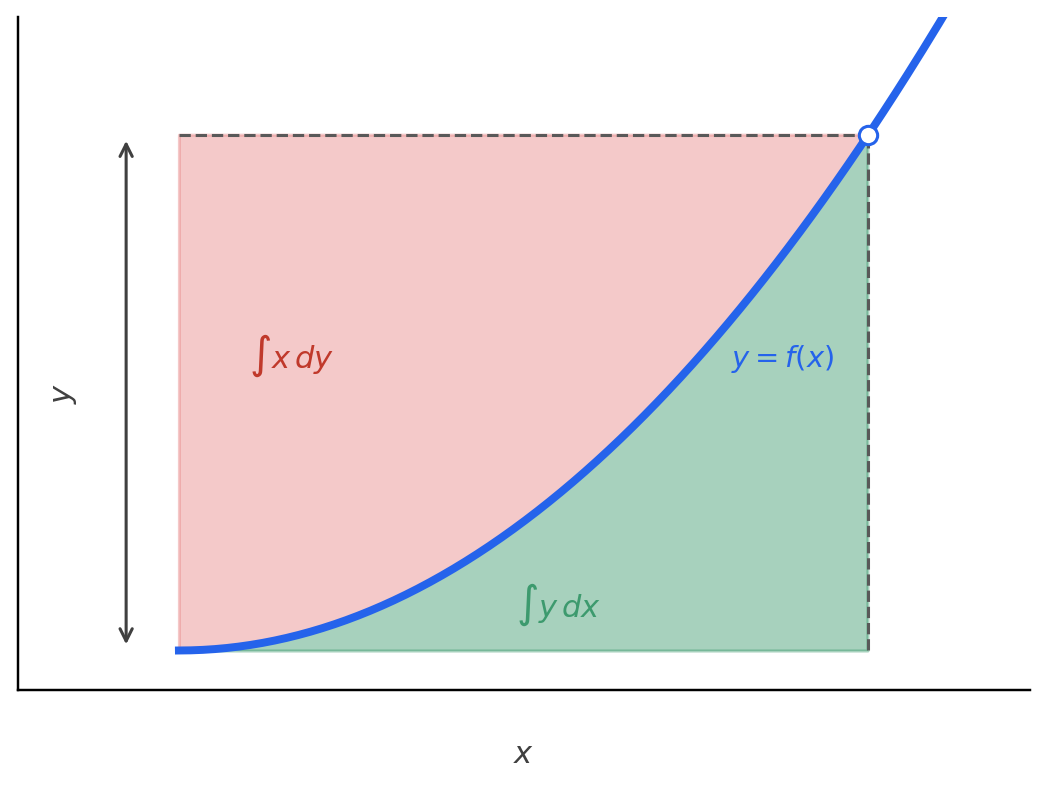
\includegraphics[width=0.62\textwidth]{figures/ibp_rectangle.png}
  \vfill
\end{frame}

\begin{frame}{2.3 Integration by parts --- example}
  \footnotesize
  \textbf{Example.}\
  $\displaystyle\int x e^x\,dx$.

  \medskip
  Let $u=x$, $dv=e^x\,dx$, so $du=dx$, $v=e^x$:
  \[
    \int x e^x\,dx
    = x e^x - \int e^x\,dx
    = x e^x - e^x + C
    = e^x(x-1)+C.
  \]

  \medskip
  \textbf{Check.}\
  $\dfrac{d}{dx}\bigl[e^x(x-1)\bigr]=e^x(x-1)+e^x=x e^x$. \checkmark
\end{frame}

\begin{frame}{2.3 PMF and CDF --- discrete example (dice)}
  \footnotesize
  \textbf{Setup.}\ Fair die: $X\in\{1,2,3,4,5,6\}$.

  \medskip
  \textbf{Probability mass function (PMF):}\
  $p(k)=P(X=k)=\tfrac16$ for $k=1,\ldots,6$.

  \medskip
  \textbf{Event (sum rule):}\
  $P(2\le X\le 4)=p(2)+p(3)+p(4)=\tfrac12$.

  \medskip
  \textbf{Cumulative distribution function (CDF):}\
  $F(x)=P(X\le x)$, defined for \textbf{all} real $x$.
  It is \textbf{right-continuous} and jumps by $p(k)$ only at mass points
  $k=1,\ldots,6$ (flat in between).

  \medskip
  Example: $F(3)=\tfrac12$ and $F(3.7)=F(3)=\tfrac12$.

  \medskip
  {\scriptsize Discrete: \textbf{PMF} and a step \textbf{CDF}.\
  Continuous (next): \textbf{PDF} and a continuous \textbf{CDF}.}
\end{frame}

\begin{frame}[plain]{2.3 PMF and CDF --- dice (graph)}
  \centering
  \vfill
  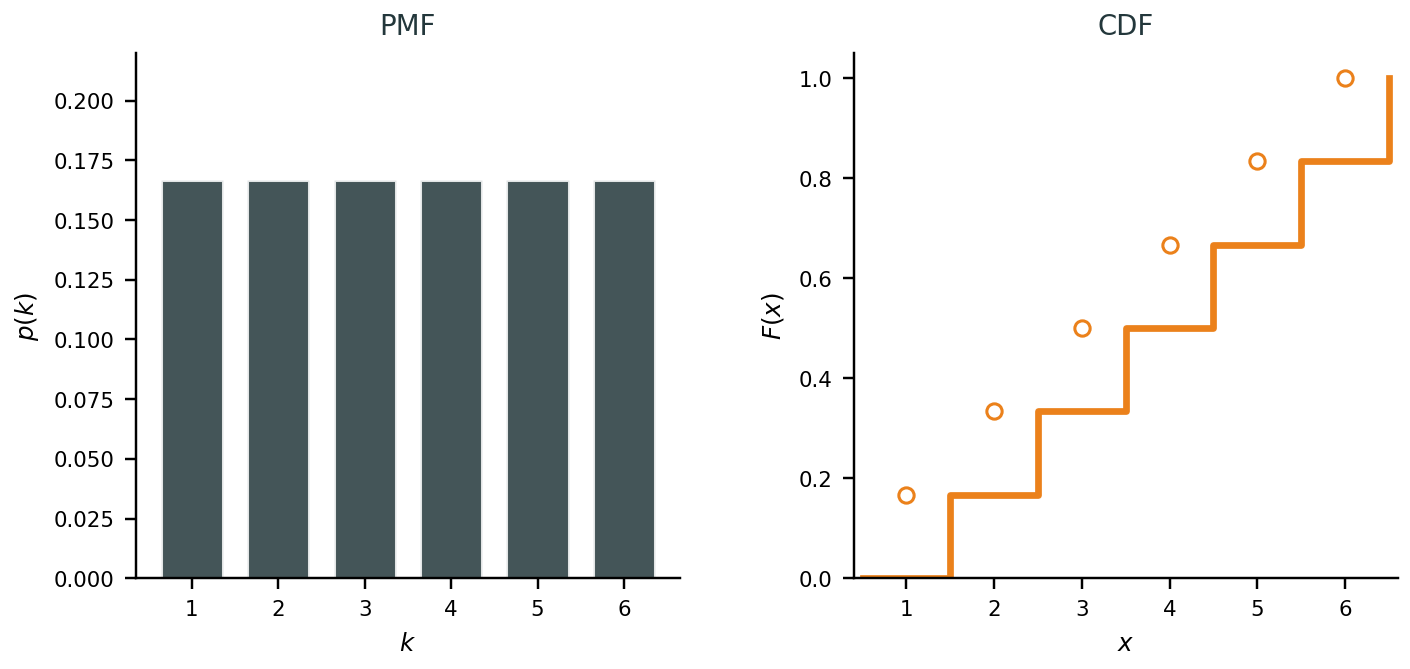
\includegraphics[width=0.88\textwidth]{figures/dice_pmf_cdf.png}
  \vfill
\end{frame}

\begin{frame}{2.3 PDF and CDF --- continuous case}
  \footnotesize
  Let $X$ be a continuous random variable.

  \medskip
  \textbf{Probability density function (PDF):}\
  $f(x)\ge 0$ and $\displaystyle\int_{-\infty}^{\infty} f(x)\,dx=1$.
  Then $P(a\le X\le b)=\displaystyle\int_a^b f(x)\,dx$.

  \medskip
  \textbf{Cumulative distribution function (CDF):}\
  $F(x)=P(X\le x)=\displaystyle\int_{-\infty}^{x} f(t)\,dt$;
  a \textbf{continuous} curve in $x$ (not jumps on a finite outcome list).

  \medskip
  \textbf{FTC:}\ if $f$ is continuous, then $F'(x)=f(x)$.
\end{frame}

\begin{frame}[plain]{2.3 PDF and CDF --- Unif$(0,1)$ (graph)}
  \centering
  \vfill
  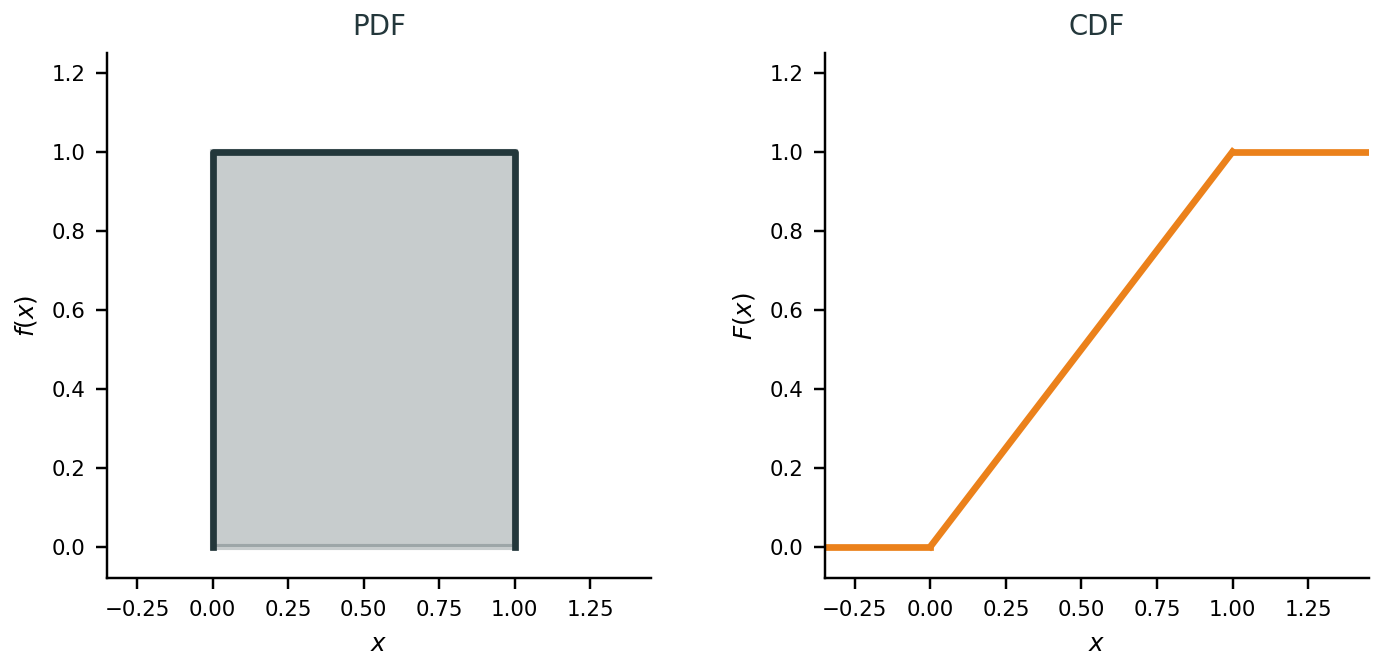
\includegraphics[width=0.88\textwidth]{figures/uniform_pdf_cdf.png}
  \vfill
\end{frame}

\begin{frame}{2.3 Expectation from the CDF}
  \footnotesize
  \begin{columns}[T,onlytextwidth]
    \column{0.48\textwidth}
    For a \textbf{non-negative} continuous $X$ with PDF $f$ and CDF $F$,
    \[
      \mathbb{E}[X]
      = \int_0^\infty x f(x)\,dx
      = \int_0^\infty \bigl(1-F(x)\bigr)\,dx.
    \]

    \smallskip
    \textbf{Intuition.}\
    For $X\sim\mathrm{Unif}(0,1)$, each vertical strip has height $1-F(x)$;
    $\mathbb{E}[X]$ is their total area.

    \medskip
    {\scriptsize Derivation via integration by parts (\InterestOnly):
    \AppendixLink{sec:expectation-cdf-proof}.}

    \column{0.50\textwidth}
    \centering
    \vspace{-0.1cm}
    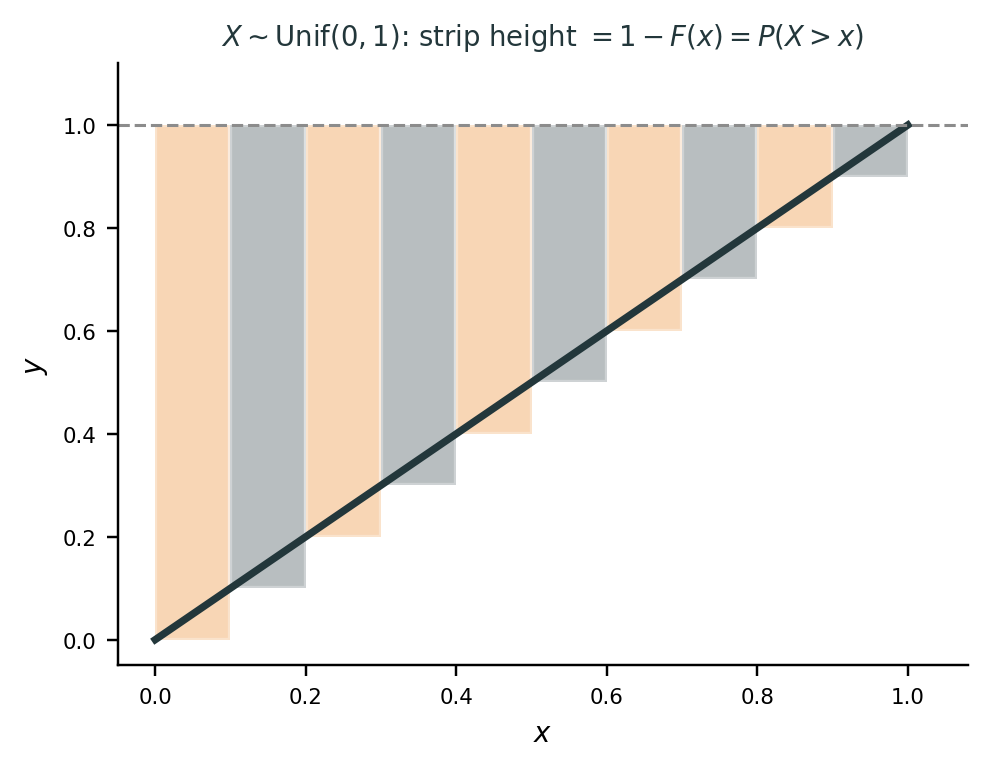
\includegraphics[width=0.96\linewidth]{figures/expectation_cdf_region.png}
  \end{columns}
\end{frame}

\begin{frame}{2.3 Variance}
  \footnotesize
  Let $\mu=\mathbb{E}[X]$. The \textbf{variance} measures average squared distance from the mean:
  \[
    \mathrm{Var}(X)
    =\mathbb{E}\bigl[(X-\mu)^2\bigr].
  \]
  (Standard deviation: $\mathrm{SD}(X)=\sqrt{\mathrm{Var}(X)}$.)

  \medskip
  \textbf{Scaling.}\ $\mathrm{Var}(aX+b)=a^2\mathrm{Var}(X)$.

  \medskip
  \textbf{Proof.}\
  $\mathbb{E}[aX+b]=a\mu+b$, so
  \[
    \mathrm{Var}(aX+b)
    =\mathbb{E}\bigl[(aX+b-a\mu-b)^2\bigr]
    =\mathbb{E}\bigl[a^2(X-\mu)^2\bigr]
    =a^2\mathrm{Var}(X).
  \]
  A shift $b$ cancels; a scale $a$ factors out as $a^2$.
\end{frame}

\begin{frame}{2.3 Why $\mathrm{Var}(X)=\mathbb{E}[X^2]-(\mathbb{E}[X])^2$}
  \footnotesize
  Expand the square:
  \[
    (X-\mu)^2
    = X^2-2\mu X+\mu^2.
  \]
  Take expectations (linearity):
  \[
    \mathrm{Var}(X)
    =\mathbb{E}[X^2]-2\mu\,\mathbb{E}[X]+\mu^2
    =\mathbb{E}[X^2]-2\mu^2+\mu^2
    =\mathbb{E}[X^2]-\mu^2.
  \]
  Since $\mu=\mathbb{E}[X]$,
  \[
    \boxed{\mathrm{Var}(X)=\mathbb{E}[X^2]-(\mathbb{E}[X])^2.}
  \]

  \medskip
  {\scriptsize Recipe: compute $\mathbb{E}[X]$ and $\mathbb{E}[X^2]$, then subtract.
  For Unif$(0,1)$: $\mathbb{E}[X]=\tfrac12$, $\mathbb{E}[X^2]=\tfrac13$, so
  $\mathrm{Var}(X)=\tfrac13-\tfrac14=\tfrac{1}{12}$.}
\end{frame}

\begin{frame}{2.3 Joint distributions}
  \footnotesize
  For two random variables $(X,Y)$:

  \medskip
  \textbf{Discrete.}\ Joint PMF $p(x,y)=P(X=x,Y=y)$.
  Marginals: $p_X(x)=\sum_y p(x,y)$, $p_Y(y)=\sum_x p(x,y)$.

  \medskip
  \textbf{Continuous.}\ Joint PDF $f(x,y)\ge 0$ with
  $\displaystyle\iint f(x,y)\,dx\,dy=1$.
  Marginals: $f_X(x)=\displaystyle\int f(x,y)\,dy$, etc.

  \medskip
  \textbf{Independence.}\
  $p(x,y)=p_X(x)p_Y(y)$ (or $f(x,y)=f_X(x)f_Y(y)$).
  Then knowing $X$ tells you nothing about $Y$.

  \medskip
  {\scriptsize Economics: prices and quantities, type and signal, income and hours ---
  almost never independent.}
\end{frame}

\begin{frame}{2.3 Conditional probability}
  \footnotesize
  \textbf{Definition.}\ If $P(B)>0$,
  \[
    P(A\mid B)=\frac{P(A\cap B)}{P(B)}.
  \]
  Read: probability of $A$ \textbf{given} that $B$ occurred.

  \medskip
  \textbf{Discrete conditional PMF.}\
  $p(y\mid x)=P(Y=y\mid X=x)=\dfrac{p(x,y)}{p_X(x)}$ when $p_X(x)>0$.

  \medskip
  \textbf{Continuous.}\
  $f(y\mid x)=\dfrac{f(x,y)}{f_X(x)}$.

  \medskip
  \textbf{Conditional expectation.}\
  $\mathbb{E}[Y\mid X=x]=\sum_y y\,p(y\mid x)$
  (or $\displaystyle\int y f(y\mid x)\,dy$).
  As a random variable: $\mathbb{E}[Y\mid X]$.
\end{frame}

\begin{frame}{2.3 Bayes --- prior and posterior}
  \footnotesize
  \textbf{Bayes' rule.}\
  \[
    P(A\mid B)
    =\frac{P(B\mid A)\,P(A)}{P(B)}.
  \]
  \textbf{Prior} $P(A)$: belief before seeing data.
  \textbf{Likelihood} $P(B\mid A)$: how the data arise if $A$ is true.
  \textbf{Posterior} $P(A\mid B)$: updated belief after seeing $B$.

  \medskip
  Denominator (law of total probability):
  \[
    P(B)=P(B\mid A)P(A)+P(B\mid A^c)P(A^c).
  \]

  \medskip
  \textbf{Economics.}\
  Prior on type / quality / state; observe a signal; form a posterior and act.
\end{frame}

\begin{frame}{2.3 Bayes --- worked example}
  \footnotesize
  \textbf{Setup.}\ Prevalence $P(\text{Covid})=\tfrac{1}{100}$.
  A test has sensitivity $P(+\mid \text{Covid})=\tfrac{99}{100}$
  and false-positive rate $P(+\mid \text{no Covid})=\tfrac{1}{100}$.
  You test positive. What is $P(\text{Covid}\mid +)$?

  \medskip
  \[
    P(+)
    =\tfrac{99}{100}\cdot\tfrac{1}{100}+\tfrac{1}{100}\cdot\tfrac{99}{100}
    =\tfrac{198}{10000},
    \qquad
    P(\text{Covid}\mid +)
    =\frac{(\tfrac{99}{100})(\tfrac{1}{100})}{\tfrac{198}{10000}}
    =\tfrac12.
  \]

  \medskip
  Prior $\tfrac{1}{100}$ $\to$ posterior $\tfrac12$:
  even a 99\%-accurate test leaves a 50--50 chance when the disease is rare.
\end{frame}

\begin{frame}{2.3 Intuition --- averaging group averages}
  \footnotesize
  \textbf{Example.}\ Wages $Y$ and education $X\in\{H,L\}$ (high / low).
  Suppose half the workers are high education:
  \[
    \mathbb{E}[Y\mid X=H]=60,
    \qquad
    \mathbb{E}[Y\mid X=L]=40,
    \qquad
    P(X=H)=P(X=L)=\tfrac12.
  \]

  \medskip
  Overall average wage:
  \[
    \mathbb{E}[Y]
    =\tfrac12\cdot 60+\tfrac12\cdot 40
    =50
    =\mathbb{E}\bigl[\mathbb{E}[Y\mid X]\bigr].
  \]

  \medskip
  \textbf{Intuition.}\
  The grand mean is the \textbf{weighted average of subgroup means},
  with weights equal to group shares.
  That is the law of iterated expectations before the formula.
\end{frame}

\begin{frame}{2.3 Law of iterated expectations}
  \footnotesize
  \textbf{LIE.}\
  \[
    \mathbb{E}\bigl[\mathbb{E}[Y\mid X]\bigr]=\mathbb{E}[Y].
  \]
  Averaging the conditional means recovers the unconditional mean.

  \medskip
  \textbf{Discrete proof idea.}\
  \[
    \mathbb{E}\bigl[\mathbb{E}[Y\mid X]\bigr]
    =\sum_x \mathbb{E}[Y\mid X=x]\,P(X=x)
    =\sum_x\sum_y y\,p(y\mid x)\,p_X(x)
    =\sum_y y\,p_Y(y)
    =\mathbb{E}[Y].
  \]

  \medskip
  \textbf{Use.}\
  Forecasts: if $\mathbb{E}[Y\mid X]$ is your best predictor given $X$,
  the average forecast equals the average outcome.
\end{frame}

\begin{frame}{2.3 Monty Hall --- setup}
  \footnotesize
  \textbf{Game.}\ Three doors; car behind one, goats behind the other two.
  You pick door~1. Host (who knows where the car is) always opens a different door
  with a goat --- say door~3. Should you switch to door~2?

  \medskip
  \textbf{Prior.}\ $C_i=\{\text{car behind door }i\}$, $P(C_i)=\tfrac13$ for $i=1,2,3$.

  \medskip
  \textbf{Host's rule.}\ Never opens your door; never opens the car;
  if indifferent, randomize 50--50.
  Data: $H_3=\{\text{host opens door~3}\}$.
\end{frame}

\begin{frame}{2.3 Monty Hall --- intuition}
  \footnotesize
  At the start, $P(C_1)=\tfrac13$ and
  \[
    P(C_2\cup C_3)=\tfrac23.
  \]

  \medskip
  Seeing the host open door~3 does \textbf{not} change anything about your pick:
  the host never opens door~1, so that reveal is not news about $C_1$.
  Thus $P(C_1\mid H_3)$ stays $\tfrac13$.

  \medskip
  The other two doors still carry total probability $\tfrac23$.
  The host just showed door~3 is a goat, so $C_3$ is impossible.
  All of that $\tfrac23$ therefore piles onto the remaining closed door:
  \[
    P(C_2\mid H_3)=\tfrac23.
  \]
  Switch.
\end{frame}

\begin{frame}{2.3 Monty Hall --- 100 doors}
  \footnotesize
  Same game with \textbf{100 doors}. You pick door~1
  ($P=\tfrac{1}{100}$). The other 99 doors share $\tfrac{99}{100}$.

  \medskip
  Host opens 98 goat doors among those 99, leaving door~37 closed.
  Your door is still probability $\tfrac{1}{100}$
  (host never opens it, so no news about it).

  \medskip
  The bundle of 99 doors still has $\tfrac{99}{100}$;
  98 of them are now open goats, so that whole mass falls on door~37:
  \[
    P(\text{car behind 37}\mid\text{host leaves 37})
    =\frac{99}{100}.
  \]

  \medskip
  Switching is almost surely right. The 3-door case is the same logic with a smaller pile.
\end{frame}

\THFrame{2.3 Monty Hall --- Bayes solution}
  \footnotesize
  \textbf{Exercise.}\ Uniform prior $P(C_i)=\tfrac13$. You pick door~1; host opens door~3.
  Using Bayes' rule, compute $P(C_1\mid H_3)$ and $P(C_2\mid H_3)$. Switch or stay?

  \medskip
  \textbf{Solution.}\ Likelihoods:
  $P(H_3\mid C_1)=\tfrac12$, $P(H_3\mid C_2)=1$, $P(H_3\mid C_3)=0$.
  \[
    P(H_3)
    =\tfrac12\cdot\tfrac13+1\cdot\tfrac13+0\cdot\tfrac13
    =\tfrac12.
  \]
  \[
    P(C_1\mid H_3)=\frac{(\tfrac12)(\tfrac13)}{\tfrac12}=\tfrac13,
    \qquad
    P(C_2\mid H_3)=\frac{1\cdot\tfrac13}{\tfrac12}=\tfrac23.
  \]
  Switch --- same answer as the intuition.
\end{frame}

\section{2.4 --- Leibniz Rule and Fubini}

\begin{frame}{2.4 Leibniz rule --- fixed limits}
  \footnotesize
  \textbf{Setup.}\ $F(\theta)=\displaystyle\int_a^b f(x,\theta)\,dx$ with fixed $a,b$.

  \medskip
  \textbf{Leibniz rule (fixed limits).}\
  When regularity holds,
  \[
    \frac{dF}{d\theta}
    = \int_a^b \frac{\partial f}{\partial \theta}(x,\theta)\,dx.
  \]

  \medskip
  \textbf{Regularity (enough for this camp).}\
  \begin{itemize}
    \item $\dfrac{\partial f}{\partial \theta}(x,\theta)$ exists
    \item $f$ and $\dfrac{\partial f}{\partial \theta}$ are \textbf{continuous} in $(x,\theta)$
  \end{itemize}
  Then you may swap $\dfrac{d}{d\theta}$ and $\displaystyle\int_a^b$.

  \medskip
  \textbf{Idea.}\ Only the integrand moves with $\theta$; the limits $a,b$ stay fixed.

  \medskip
  {\scriptsize When regularity fails (\InterestOnly):
  \AppendixLink{sec:leibniz-failure}.}
\end{frame}

\begin{frame}{2.4 Leibniz rule --- variable limits}
  \footnotesize
  \textbf{Setup.}\
  $F(\theta)=\displaystyle\int_{a(\theta)}^{b(\theta)} f(x,\theta)\,dx$.

  \medskip
  \textbf{Leibniz rule (variable limits).}\
  When $a(\theta)$, $b(\theta)$ are differentiable and regularity holds,
  \[
    \frac{dF}{d\theta}
    = f\bigl(b(\theta),\theta\bigr)\,b'(\theta)
      - f\bigl(a(\theta),\theta\bigr)\,a'(\theta)
      + \int_{a(\theta)}^{b(\theta)}
        \frac{\partial f}{\partial \theta}(x,\theta)\,dx.
  \]

  \medskip
  \textbf{Three parts.}\
  \textbf{(i)} area added/lost at the \textbf{upper} limit $b$;\
  \textbf{(ii)} at the \textbf{lower} limit $a$;\
  \textbf{(iii)} change \textbf{inside} the interval ($\partial f/\partial\theta$).

  \medskip
  {\scriptsize Graph on next slide: grey $=$ $\partial f/\partial\theta$;\
  pink/blue $=$ lower/upper limit terms ($a'(\theta)$, $b'(\theta)$).}
\end{frame}

\begin{frame}[plain]{2.4 Leibniz rule --- variable limits (graph)}
  \centering
  \vfill
  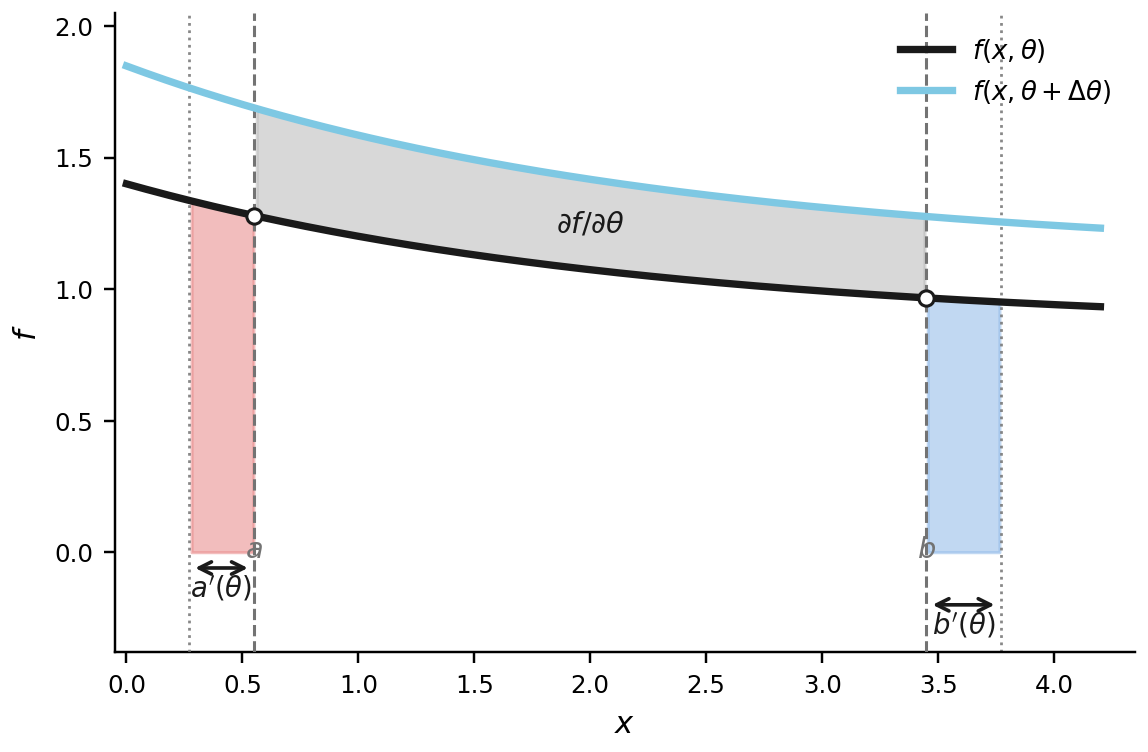
\includegraphics[width=0.78\textwidth]{figures/leibniz_variable_limits.png}
  \vfill
\end{frame}

\begin{frame}{2.4 Leibniz --- practice (monopoly pricing)}
  \footnotesize
  \textbf{Economic setup.}\
  A unit mass of consumers; consumer $i$ has willingness to pay $v_i$, with
  $v_i\sim F$ (cdf $F$, pdf $f$ on $[0,\bar v]$).
  A monopolist sets price $p$; $i$ buys iff $v_i\ge p$.

  \medskip
  \textbf{Type-dependent cost.}\
  Serving type $v$ costs $c(v)$ (e.g.\ quality, personalization, delivery).
  Profit from a buyer with valuation $v\ge p$ is $p-c(v)$ --- margin \textbf{varies by type}.

  \medskip
  \textbf{Total profit (no simple closed form).}\
  \[
    \pi(p)=\int_p^{\bar v}\bigl(p-c(v)\bigr)\,f(v)\,dv
    \qquad\text{(cannot write as $(p-c)(1-F(p))$ when $c=c(v)$).}
  \]
  The lower limit moves with $p$ --- \textbf{Leibniz is the right tool}.

  \medskip
  \textbf{Practice.}\
  Find $\dfrac{d\pi}{dp}$ and interpret each term.
  {\scriptsize If $c$ is constant, product rule also works; here it does not.}
\end{frame}

\begin{frame}{2.4 Leibniz --- practice solution (monopoly pricing)}
  \footnotesize
  \textbf{Apply variable-limits Leibniz to $\pi(p)$ directly.}\
  Lower limit $a(p)=p$, upper limit $\bar v$; only $p$ in the integrand is the leading $p$:
  \[
    \frac{d\pi}{dp}
    = -\bigl(p-c(p)\bigr)f(p)\,a'(p)
      + \int_p^{\bar v}
        \frac{\partial}{\partial p}\bigl[(p-c(v))f(v)\bigr]\,dv.
  \]

  \medskip
  \textbf{Simplify.}\
  $a'(p)=1$;\ $\dfrac{\partial}{\partial p}\bigl[(p-c(v))f(v)\bigr]=f(v)$ (since $c(v)$ does not depend on $p$):
  \[
    \frac{d\pi}{dp}
    = -\bigl(p-c(p)\bigr)f(p)
      + \int_p^{\bar v} f(v)\,dv
    = -\bigl(p-c(p)\bigr)f(p) + \bigl(1-F(p)\bigr).
  \]

  \medskip
  \textbf{Economic reading.}\
  \begin{itemize}
    \item \textbf{Lower limit} $-\bigl(p-c(p)\bigr)f(p)$: lose margin $p-c(p)$ on the marginal buyer ($v=p$).
    \item \textbf{Inside} $1-F(p)$: raising $p$ still adds $1\cdot dp$ profit on \textbf{each} remaining buyer.
  \end{itemize}

  \medskip
  {\scriptsize\textbf{FOC.}\
  $\bigl(p-c(p)\bigr)f(p)=1-F(p)$;
  constant $c$ gives the usual markup rule $p-c=\dfrac{1-F(p)}{f(p)}$.}
\end{frame}

\begin{frame}{2.4 Fubini's theorem}
  \footnotesize
  \textbf{Statement.}\
  If $f$ is \textbf{integrable} on region $D$, i.e.
  \[
    \iint_D \lvert f(x,y)\rvert\,dx\,dy < \infty,
  \]
  then
  \[
    \iint_D f(x,y)\,dx\,dy
    = \int\!\left(\int f(x,y)\,dx\right)dy
    = \int\!\left(\int f(x,y)\,dy\right)dx,
  \]
  (inner limits depend on the shape of $D$).

  \medskip
  \textbf{Camp shortcut.}\
  If $D$ is bounded and $f$ is \textbf{continuous} on $D$, then $f$ is integrable
  and Fubini applies.

  \medskip
  {\scriptsize Tonelli (for interest): if $f\ge 0$ and measurable, the same swap holds
  without checking $\iint\lvert f\rvert$ first.}
\end{frame}

\begin{frame}{2.4 Fubini --- triangle example}
  \footnotesize
  \textbf{Example (triangle).}\
  \[
    D=\{(x,y): 0\le x\le 1,\; 0\le y\le x\}.
  \]

  \medskip
  Compute $\displaystyle\iint_D (x+y)\,dx\,dy$.

  \medskip
  \textbf{$y$ first, then $x$:}\ for fixed $x$, $y\in[0,x]$:
  \[
    \int_0^1\!\int_0^x (x+y)\,dy\,dx
    = \int_0^1 \Bigl[xy+\tfrac{y^2}{2}\Bigr]_{0}^{x}dx
    = \int_0^1 \tfrac{3x^2}{2}\,dx
    = \tfrac12.
  \]

  \medskip
  \textbf{$x$ first, then $y$:}\ for fixed $y$, $x\in[y,1]$:
  \[
    \int_0^1\!\int_y^1 (x+y)\,dx\,dy
    = \int_0^1 \Bigl[\tfrac{x^2}{2}+xy\Bigr]_{y}^{1}dy
    = \int_0^1 \Bigl(\tfrac12+y-\tfrac{3y^2}{2}\Bigr)dy
    = \tfrac12.
  \]

  \medskip
  {\scriptsize Graph on next slide: same triangle, different slice directions.}
\end{frame}

\begin{frame}[plain]{2.4 Fubini --- triangle (graph)}
  \centering
  \vfill
  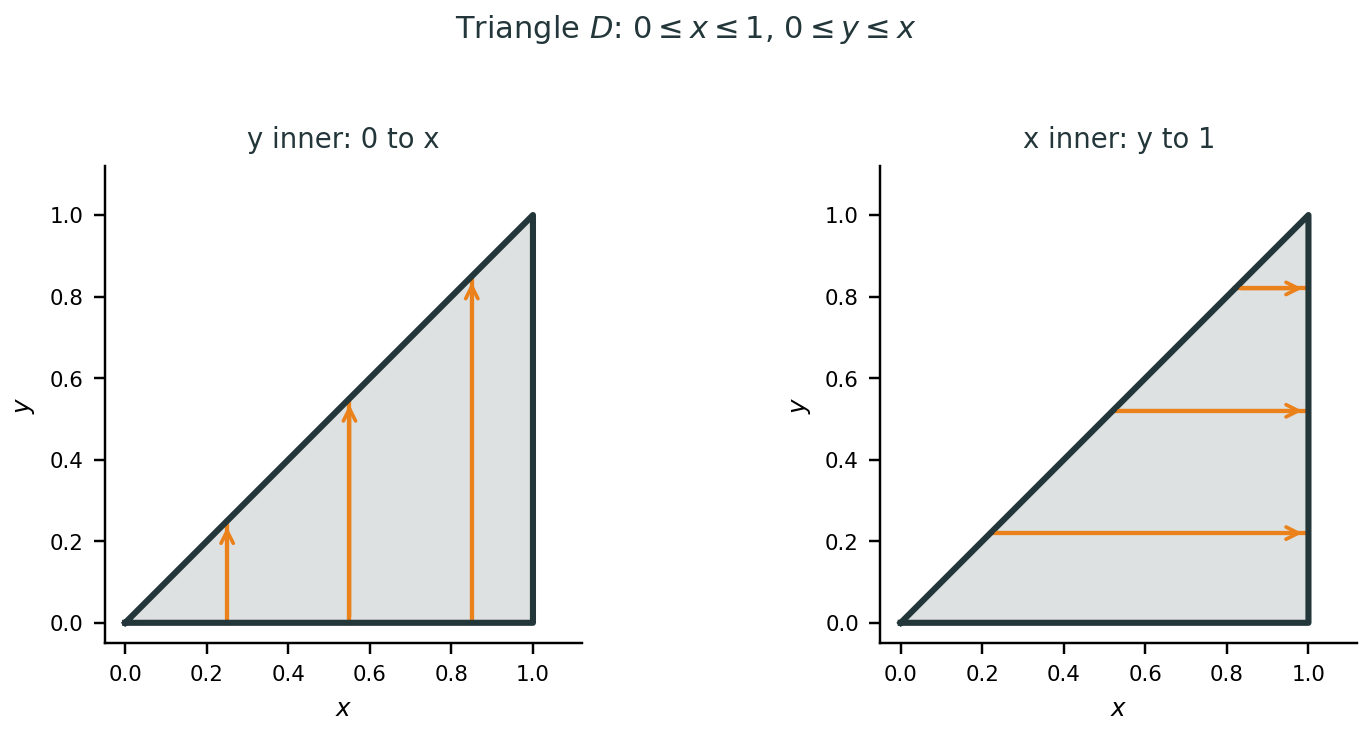
\includegraphics[width=0.88\textwidth]{figures/fubini_triangle.png}
  \vfill
\end{frame}

\begin{frame}{2.4 Fubini --- practice (between two curves)}
  \footnotesize
  \textbf{Region (non-rectangular).}\
  Between the parabola $y=x^2$ and the line $y=x$ on $[0,1]$:
  \[
    D=\{(x,y):\ 0\le x\le 1,\ x^2\le y\le x\}.
  \]
  (On $(0,1)$, the line lies \textbf{above} the parabola.)

  \medskip
  \textbf{Practice.}\
  Compute $\displaystyle\iint_D xy\,dx\,dy$ using Fubini \textbf{twice} (different inner variable).

  \medskip
  \textbf{Slice limits to find.}\
  \begin{itemize}
    \item \textbf{$y$ inner:}\ for fixed $x\in[0,1]$, $y$ runs from $x^2$ to $x$.
    \item \textbf{$x$ inner:}\ for fixed $y\in[0,1]$, solve $x^2\le y\le x$ to get $x\in[y,\sqrt{y}]$.
  \end{itemize}

  \medskip
  {\scriptsize Graph on next slide; detailed solution on the following slides.}
\end{frame}

\begin{frame}[plain]{2.4 Fubini --- practice (graph)}
  \centering
  \vfill
  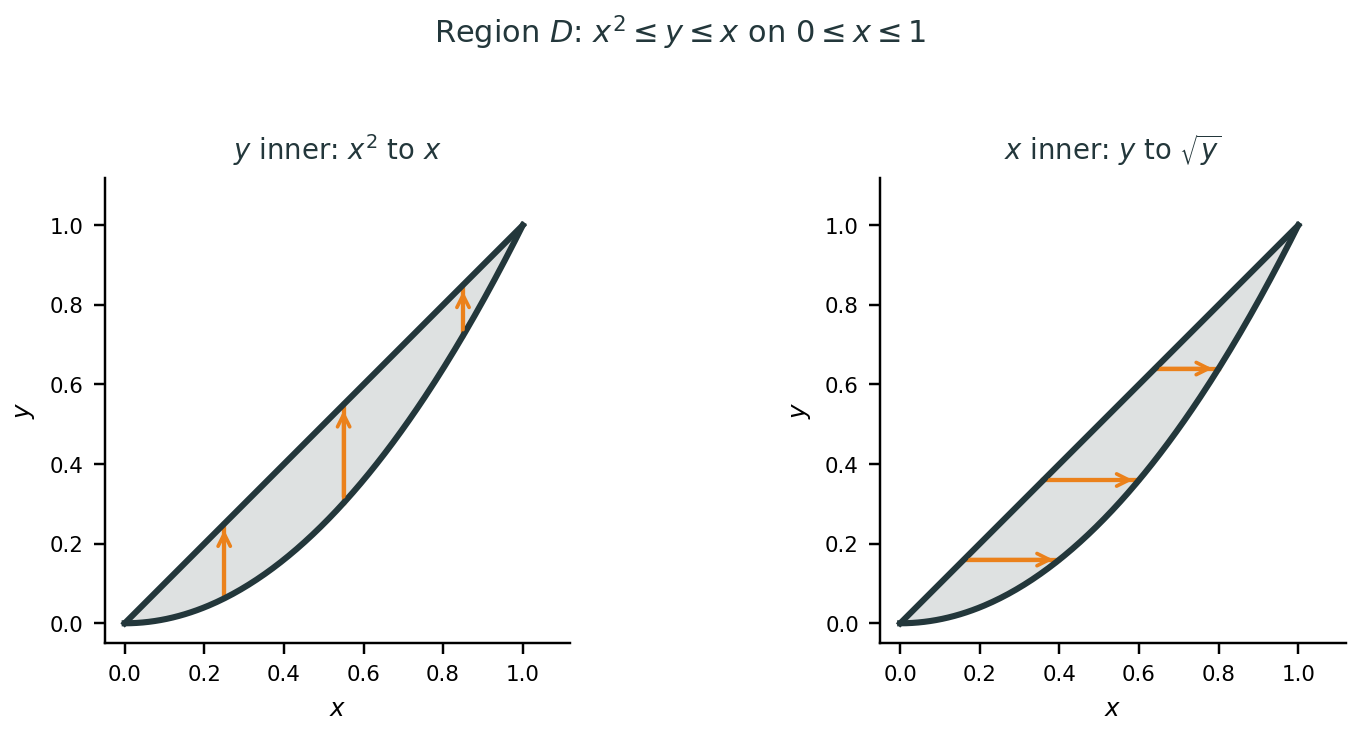
\includegraphics[width=0.88\textwidth]{figures/fubini_parabola_line.png}
  \vfill
\end{frame}

\begin{frame}{2.4 Fubini --- practice solution ($y$ inner first)}
  \footnotesize
  \textbf{Order 1:}\ $\displaystyle\int_0^1\!\int_{x^2}^{x} xy\,dy\,dx$.

  \medskip
  \textbf{Inner integral (fix $x$).}\
  \[
    \int_{x^2}^{x} xy\,dy
    = x\left[\frac{y^2}{2}\right]_{y=x^2}^{y=x}
    = x\left(\frac{x^2}{2}-\frac{x^4}{2}\right)
    = \frac{x^3}{2}-\frac{x^5}{2}.
  \]

  \medskip
  \textbf{Outer integral.}\
  \[
    \int_0^1 \left(\frac{x^3}{2}-\frac{x^5}{2}\right)dx
    = \left[\frac{x^4}{8}-\frac{x^6}{12}\right]_0^1
    = \frac18-\frac{1}{12}
    = \frac{1}{24}.
  \]
\end{frame}

\begin{frame}{2.4 Fubini --- practice solution ($x$ inner first)}
  \footnotesize
  \textbf{Order 2:}\ $\displaystyle\int_0^1\!\int_{y}^{\sqrt{y}} xy\,dx\,dy$.

  \medskip
  \textbf{Why $x\in[y,\sqrt{y}]$?}\
  For fixed $y$, need $y\le x$ (from $y\le x$) and $x^2\le y$ (from $y\ge x^2$), i.e.\ $x\le\sqrt{y}$.

  \medskip
  \textbf{Inner integral (fix $y$).}\
  \[
    \int_{y}^{\sqrt{y}} xy\,dx
    = y\left[\frac{x^2}{2}\right]_{x=y}^{x=\sqrt{y}}
    = y\left(\frac{y}{2}-\frac{y^2}{2}\right)
    = \frac{y^2}{2}-\frac{y^3}{2}.
  \]

  \medskip
  \textbf{Outer integral.}\
  \[
    \int_0^1 \left(\frac{y^2}{2}-\frac{y^3}{2}\right)dy
    = \left[\frac{y^3}{6}-\frac{y^4}{8}\right]_0^1
    = \frac16-\frac18
    = \frac{1}{24}.
  \]

  \medskip
  \textbf{Check.}\
  Both orders agree --- Fubini is consistent when the region and integrand are well behaved.
\end{frame}

\section{2.5 --- Taylor Expansion and Linearization}

\begin{frame}{2.5 Taylor expansion --- formal statement}
  \footnotesize
  \textbf{One variable.}\
  If $f$ has $n$ derivatives at $a$,
  \[
    f(a+h)
    = \sum_{k=0}^{n}\frac{f^{(k)}(a)}{k!}\,h^k + R_n(h),
    \qquad R_n(h)\to 0 \text{ faster than } h^n.
  \]

  \medskip
  \textbf{Several variables} ($f\colon\mathbb R^m\to\mathbb R$, $\mathbf{a}\in\mathbb R^m$).\
  If $f$ is $C^2$ near $\mathbf{a}$,
  \[
    f(\mathbf{a}+\mathbf{h})
    = f(\mathbf{a})
      + \nabla f(\mathbf{a})\cdot\mathbf{h}
      + \tfrac12\,\mathbf{h}^{\mathsf T}H_f(\mathbf{a})\,\mathbf{h}
      + o(\|\mathbf{h}\|^2),
  \]
  {\scriptsize $H_f(\mathbf{a})$ = Hessian at $\mathbf{a}$ (matrix of second partials).}

  \medskip
  {\scriptsize Proof (one variable):
  \AppendixLink{sec:taylor-proof} (\InterestOnly).}
\end{frame}

\begin{frame}{2.5 First-order approximation}
  \footnotesize
  \textbf{One variable} (truncate at $k=1$):
  \[
    f(a+h)\approx f(a)+f'(a)\,h.
  \]

  \medskip
  \textbf{Several variables:}
  \[
    f(\mathbf{a}+\mathbf{h})
    \approx f(\mathbf{a})+\nabla f(\mathbf{a})\cdot\mathbf{h}.
  \]
\end{frame}

\begin{frame}{2.5 Second-order approximation}
  \footnotesize
  \textbf{One variable} (truncate at $k=2$):
  \[
    f(a+h)\approx f(a)+f'(a)\,h+\tfrac12 f''(a)\,h^2.
  \]

  \medskip
  \textbf{Several variables:}
  \[
    f(\mathbf{a}+\mathbf{h})
    \approx f(\mathbf{a})
      + \nabla f(\mathbf{a})\cdot\mathbf{h}
      + \tfrac12\,\mathbf{h}^{\mathsf T}H_f(\mathbf{a})\,\mathbf{h}.
  \]

  \medskip
  \textbf{Use.}\
  Captures \textbf{curvature} (concavity, cross-partials);
  improves forecasts when the first-order term is not enough.

  \medskip
  {\scriptsize It\^o's lemma:
  \AppendixLink{sec:ito-lemma} (\InterestOnly).}
\end{frame}

\QFrame{2.5 --- First-order Taylor practice (two variables)}
  \scriptsize
  \textbf{Approximate}\ $f(1.1,1.2)$ for $f(x,y)=x^2+y$ using Taylor at $(1,1)$,\ $\mathbf{h}=(0.1,0.2)$.

  \vspace{3pt}
  \onslide<2->{\textbf{At $(1,1)$:}\ $f(1,1)=2$,\ $f_x=2$,\ $f_y=1$.}\par\medskip
  \onslide<3->{\textbf{First-order:}\ $2+2(0.1)+1(0.2)=2.4$.}\par\medskip
  \onslide<4->{\textcolor{mAccent}{Exact $f(1.1,1.2)=2.41$.}}
\end{frame}

\begin{frame}{2.5 When linearization works}
  \footnotesize
  \textbf{Works well when:}
  \begin{itemize}
    \item the shift is \textbf{small}
    \item curvature is modest ($f''$ not huge)
    \item the function is differentiable
  \end{itemize}

  \medskip
  \textbf{Fails or misleads when:}
  \begin{itemize}
    \item large shifts, kinks, or non-differentiability
    \item strong nonlinearity (e.g.\ corner solutions, thresholds)
  \end{itemize}
\end{frame}

\begin{frame}{2.5 Two variables --- matrix form unpacked \quad \HessianSkip}
  \footnotesize
  \textbf{Setup.}\ $\mathbf{a}=(a_1,a_2)$,\ $\mathbf{h}=(h_1,h_2)$:
  \[
    f(\mathbf{a}+\mathbf{h})
    \approx f(\mathbf{a})
      + \nabla f(\mathbf{a})\cdot\mathbf{h}
      + \tfrac12\,\mathbf{h}^{\mathsf T}H_f(\mathbf{a})\,\mathbf{h}.
  \]

  \medskip
  \textbf{First-order.}\
  $\nabla f=(f_{x_1},f_{x_2})$ at $\mathbf{a}$, so
  $\nabla f\cdot\mathbf{h}=f_{x_1}h_1+f_{x_2}h_2$.

  \medskip
  \textbf{Second-order.}\
  {\scriptsize
  $H_f=
  \begin{pmatrix}f_{x_1x_1}&f_{x_1x_2}\\f_{x_2x_1}&f_{x_2x_2}\end{pmatrix}$,
  }
  and multiply:
  {\scriptsize
  \[
    \mathbf{h}^{\mathsf T}H_f\mathbf{h}
    = (h_1\ h_2)
      \begin{pmatrix}f_{x_1x_1}h_1+f_{x_1x_2}h_2\\
                     f_{x_2x_1}h_1+f_{x_2x_2}h_2\end{pmatrix}
    = f_{x_1x_1}h_1^2 + (f_{x_1x_2}+f_{x_2x_1})h_1h_2 + f_{x_2x_2}h_2^2.
  \]
  }
  If $f\in C^2$, then $f_{x_1x_2}=f_{x_2x_1}$, hence
  \[
    f(\mathbf{a}+\mathbf{h})
    \approx f(\mathbf{a})
      + f_{x_1}h_1 + f_{x_2}h_2
      + \tfrac12\bigl(
        f_{x_1x_1}h_1^2 + 2f_{x_1x_2}h_1h_2 + f_{x_2x_2}h_2^2
      \bigr).
  \]
\end{frame}

\begin{frame}{2.5 --- Second-order Taylor practice (two variables) \quad {\small\textcolor{mAccent}{Take home}} \quad \HessianSkip}
  \footnotesize
  \textbf{Approximate}\ $f(0.1,0.2)$ for $f(x,y)=\sin x+\cos y$ using a second-order Taylor expansion at $(0,0)$.

  \medskip
  Use $\mathbf{h}=(0.1,0.2)$ and the explicit second-order formula on the matrix-form slide.

  \medskip
  {\scriptsize Check your answer with a calculator (no need to simplify trig decimals).}
\end{frame}

\section{2.6 --- Uniform Convergence}

\begin{frame}{2.6 Pointwise vs.\ uniform convergence}
  \footnotesize
  \textbf{Pointwise.}\ $f_n\to f$ on $D$ means: for each fixed $x\in D$,
  \[
    f_n(x)\to f(x)\quad\text{as }n\to\infty.
  \]
  Equivalently: for each $x$ and every $\varepsilon>0$, $\exists\,N$ (may depend on
  \textbf{both $x$ and $\varepsilon$}) such that $|f_n(x)-f(x)|<\varepsilon$ for all $n\ge N$.

  \medskip
  \textbf{Uniform.}\ For every $\varepsilon>0$, $\exists\,N$ (depends on \textbf{$\varepsilon$ only})
  such that for all $n\ge N$ and \textbf{all} $x\in D$,
  \[
    |f_n(x)-f(x)|<\varepsilon.
  \]
  One $N$ works \textbf{uniformly} over the whole domain.
\end{frame}

\begin{frame}[plain]{2.6 Example --- pointwise but not uniform}
  \centering
  \vfill
  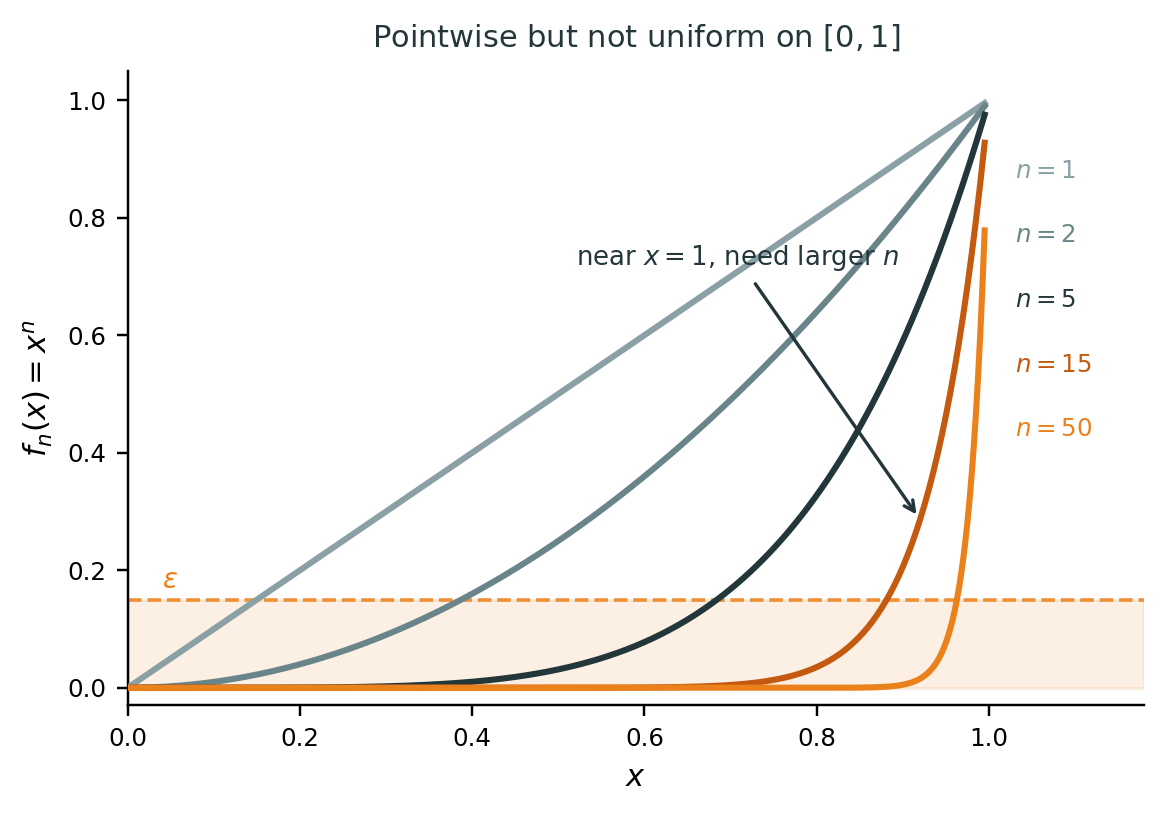
\includegraphics[width=0.82\textwidth]{figures/pointwise_not_uniform.png}
  \vfill
\end{frame}

\begin{frame}{2.6 Why uniform convergence matters}
  \footnotesize
  \textbf{Uniform convergence is the safe condition} for swapping limits with other operations:

  \medskip
  \begin{itemize}
    \item \textbf{Continuity:}\ if each $f_n$ is continuous and $f_n\to f$ \textbf{uniformly},
      then $f$ is continuous.
    \item \textbf{Integration:}\ under uniform convergence,
      $\displaystyle\lim_{n\to\infty}\int f_n=\int\lim_{n\to\infty} f_n$.
    \item \textbf{Differentiation} (with extra hypotheses): uniform convergence of derivatives
      can justify $\dfrac{d}{dx}\lim f_n=\lim\dfrac{d}{dx}f_n$.
    \item \textbf{Example ($x^n$ on $[0,1]$):}\ each $f_n$ is continuous, but the pointwise limit
      ($0$ on $[0,1)$, $1$ at $x=1$) jumps at $x=1$ --- \textbf{continuity fails} without uniform convergence.
  \end{itemize}
\end{frame}

\appendix

\begin{frame}{Appendix}
  \small
  \textbf{Not required for Math Camp.}\
  Proofs and extra examples linked from the main slides.
\end{frame}

\section{Implicit Function Theorem --- several variables}

\begin{frame}{A.1 IFT --- several variables}
  \hypertarget{sec:ift-multivar}{}
  \footnotesize
  \textbf{System:}\ $\mathbf{F}(\mathbf{y},\boldsymbol{\theta})=\mathbf{0}$,
  $\mathbf{F}\colon\mathbb{R}^{n+m}\to\mathbb{R}^n$.

  \medskip
  If the $n\times n$ Jacobian $\dfrac{\partial \mathbf{F}}{\partial \mathbf{y}}$
  is invertible at the point, then locally
  $\mathbf{y}=\mathbf{y}^*(\boldsymbol{\theta})$ and
  \[
    \frac{\partial \mathbf{y}^*}{\partial \boldsymbol{\theta}}
    =
    -\left(\frac{\partial \mathbf{F}}{\partial \mathbf{y}}\right)^{-1}
    \frac{\partial \mathbf{F}}{\partial \boldsymbol{\theta}}.
  \]

  \medskip
  {\scriptsize Same pattern as the one-variable formulas with $F_y$ and $F_\theta$.
  Appears in graduate micro; camp focus is the scalar case in section~2.1.}
\end{frame}

\section{Weierstrass EVT --- proof}

\begin{frame}{A.2 Proof.\ EVT on $[a,b]$}
  \hypertarget{sec:weierstrass-proof}{}
  \footnotesize
  \InterestOnly

  \medskip
  \textbf{Claim.}\ If $f$ is continuous on $[a,b]$, then $f$ attains a maximum and minimum on $[a,b]$.

  \medskip
  \textbf{Bolzano--Weierstrass Theorem.}\
  Every bounded sequence in $\mathbb{R}$ has a convergent subsequence.

  \medskip
  \textbf{Step 1.}\ $f$ is bounded on $[a,b]$.\
  Assume, for contradiction, that $f$ is unbounded.
  Then $\exists\,(x_n)$ in $[a,b]$ with $|f(x_n)|>n$ for all $n$.
  The sequence $(x_n)$ is bounded (it lies in $[a,b]$).
  By Bolzano--Weierstrass, some subsequence $(x_{n_k})$ converges to $c\in[a,b]$.
  Continuity gives $f(x_{n_k})\to f(c)$.
  But $|f(x_{n_k})|>n_k\to\infty$, a contradiction.
  Hence $f$ is bounded; let $M=\sup\{f(x):x\in[a,b]\}$.
\end{frame}

\begin{frame}{A.2 Proof.\ EVT on $[a,b]$ (continued)}
  \footnotesize
  \textbf{Step 2 --- claim.}\
  $f$ attains its maximum $M=\sup\{f(x):x\in[a,b]\}$ on $[a,b]$;
  i.e.\ $\exists\,d\in[a,b]$ with $f(d)=M$.

  \medskip
  \textbf{Why $\exists\,(y_n)$ in $[a,b]$ with $f(y_n)\to M$.}\
  By definition of supremum:
  \begin{enumerate}
    \item $f(x)\le M$ for all $x\in[a,b]$;
    \item for every $\varepsilon>0$, $\exists\,x\in[a,b]$ with $f(x)>M-\varepsilon$.
  \end{enumerate}
  Take $\varepsilon_n=\tfrac1n$: pick $y_n\in[a,b]$ with $f(y_n)>M-\tfrac1n$.
  Since $f(y_n)\le M$,
  \[
    M-\tfrac1n < f(y_n)\le M
    \qquad\Rightarrow\qquad
    f(y_n)\to M.
  \]
\end{frame}

\begin{frame}{A.2 Proof.\ EVT on $[a,b]$ (continued)}
  \footnotesize
  \textbf{Step 2 --- finish.}

  \medskip
  \textbf{1.}\ $(y_n)$ is \textbf{bounded}: each $y_n\in[a,b]\subset\mathbb{R}$.

  \medskip
  \textbf{2.}\ By Bolzano--Weierstrass, some subsequence $(y_{n_k})$ converges to a limit
  $d\in[a,b]$.

  \medskip
  \textbf{3.}\ Since $f(y_n)\to M$, every subsequence has the \textbf{same limit}:
  \[
    f(y_{n_k})\to M.
  \]

  \medskip
  \textbf{4.}\ By \textbf{continuity} of $f$ at $d$,
  \[
    f(d)=\lim_{k\to\infty} f(y_{n_k})=M.
  \]
  So $M$ is attained at $d\in[a,b]$.
  {\scriptsize Minimum: repeat for $-f$.}
  \hfill$\square$
\end{frame}

\section{Expectation from the CDF --- proof}

\begin{frame}{A.3 Expectation from the CDF}
  \hypertarget{sec:expectation-cdf-proof}{}
  \footnotesize
  \textbf{Claim.}\ For non-negative continuous $X$ with PDF $f$ and CDF $F$,
  \[
    \mathbb{E}[X]
    = \int_0^\infty x f(x)\,dx
    = \int_0^\infty \bigl(1-F(x)\bigr)\,dx.
  \]

  \medskip
  \textbf{Proof (integration by parts).}\
  Set $u=1-F(x)$ and $dv=dx$. Then $du=-f(x)\,dx$ and $v=x$:
  \[
    \int_0^\infty (1-F(x))\,dx
    = \bigl[x(1-F(x))\bigr]_0^\infty
      - \int_0^\infty x\,(-f(x))\,dx
    = \bigl[x(1-F(x))\bigr]_0^\infty + \int_0^\infty x f(x)\,dx.
  \]

  \medskip
  At $x=0$, $x(1-F(x))=0$.
  As $x\to\infty$, $x(1-F(x))\to 0$ when $\mathbb{E}[X]<\infty$.
  Hence $\displaystyle\int_0^\infty (1-F(x))\,dx=\mathbb{E}[X]$.
  \hfill$\square$
\end{frame}

\section{Leibniz rule --- when it can fail}

\begin{frame}{A.4 Leibniz rule --- failure example}
  \hypertarget{sec:leibniz-failure}{}
  \footnotesize
  \textbf{Example (fixed limits).}\
  On $[0,1]$, let
  \[
    f(x,\theta)=\mathbf{1}\{x>\theta\}
    \qquad\text{(step jumps at }x=\theta\text{)}.
  \]

  \medskip
  Then
  \[
    F(\theta)=\int_0^1 f(x,\theta)\,dx = 1-\theta
    \quad\Rightarrow\quad
    F'(\theta)=-1.
  \]

  \medskip
  \textbf{Why Leibniz fails.}\
  The discontinuity \textbf{moves with} $\theta$, so $\partial f/\partial\theta$
  is not continuous on $[0,1]\times I$.
  Naively $\partial f/\partial\theta=0$ a.e., so
  $\displaystyle\int_0^1 0\,dx=0\neq F'(\theta)$.
\end{frame}

\begin{frame}[plain]{A.4 Leibniz failure --- moving step (graph)}
  \centering
  \vfill
  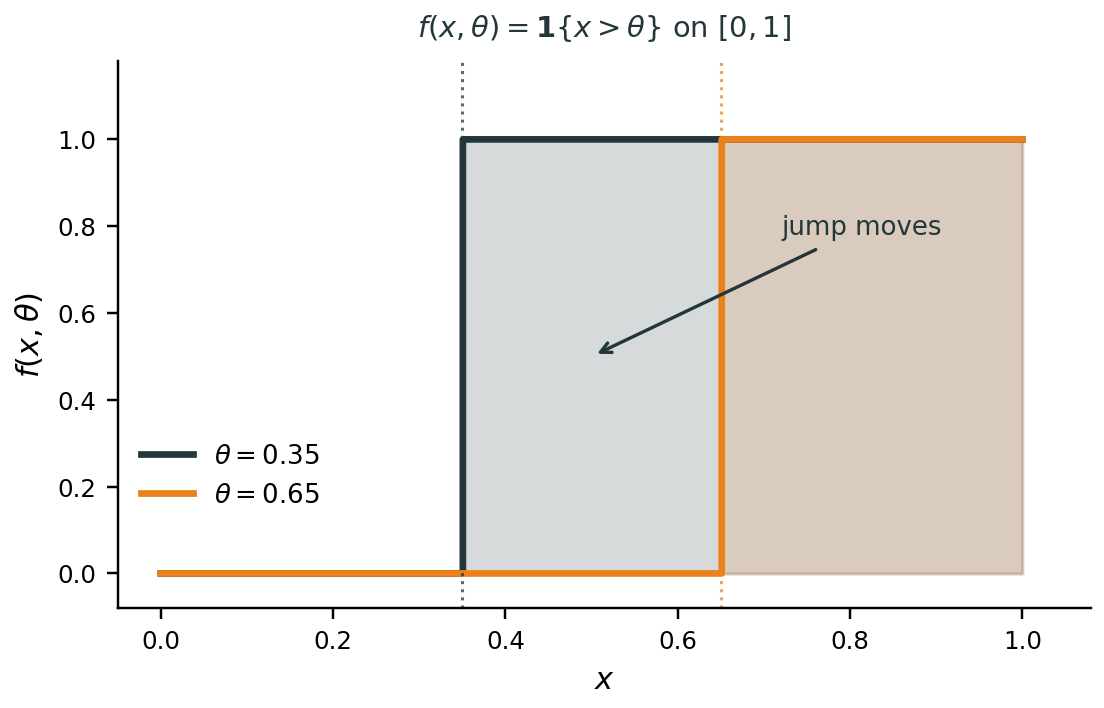
\includegraphics[width=0.78\textwidth]{figures/leibniz_failure_step.png}
  \vfill
\end{frame}

\section{Taylor expansion --- proof}

\begin{frame}{A.5 Taylor expansion (one variable)}
  \hypertarget{sec:taylor-proof}{}
  \footnotesize
  \textbf{Claim (second order).}\
  If $f\in C^2$ on an interval containing $a$ and $a+h$, then
  \[
    f(a+h)
    = f(a)+f'(a)\,h+\tfrac12 f''(c)\,h^2
  \]
  for some $c$ strictly between $a$ and $a+h$.

  \medskip
  \textbf{Proof.}\
  Write
  \[
    f(a+h)=f(a)+h f'(a)+R(h).
  \]
  \textbf{Step 1.}\
  By FTC and the chain rule,
  $f(a+h)-f(a)=\displaystyle\int_0^h f'(a+t)\,dt$, so
  \[
    R(h)=\int_0^h \bigl[f'(a+t)-f'(a)\bigr]\,dt.
  \]
  \textbf{Step 2.}\
  For each $t\in(0,h]$, MVT on $f'$ gives
  $f'(a+t)-f'(a)=t f''(c_t)$ with $c_t\in(a,a+t)$.
  Hence
  \[
    R(h)=\int_0^h t f''(c_t)\,dt
    = \tfrac{h^2}{2}\,f''(c)
  \]
  for some $c$ between $a$ and $a+h$ (continuous $f''$).
  \hfill$\square$

  \medskip
  {\scriptsize First order follows from the $n=1$ case (or MVT on $f$ directly).\
  Multivariable formulas follow from applying the chain rule along
  $\mathbf{a}+t\mathbf{h}$.}
\end{frame}

\section{Taylor and It\^o's lemma}

\begin{frame}{A.6 What is Brownian motion?}
  \footnotesize

  \textbf{Brownian motion} $W_t$ (also called a \textbf{Wiener process}):\
  a continuous-time \textbf{random} path with $W_0=0$.

  \medskip
  \textbf{Intuition.}\
  Think of a particle jolted by unpredictable shocks (e.g.\ noise in a stock price).
  You cannot forecast the next jiggle, but you can describe its \textbf{typical size}.

  \medskip
  \textbf{Key facts (informal).}
  \begin{itemize}
    \item Over $[t,t+\Delta t]$: increment $\Delta W=W_{t+\Delta t}-W_t$ has mean $0$ and variance $\Delta t$
    \item Increments on \textbf{non-overlapping} intervals are independent
    \item Paths are \textbf{continuous} but very jagged (not differentiable in the usual sense)
  \end{itemize}

  \medskip
  {\scriptsize In $dX_t=\mu\,dt+\sigma\,dW_t$, the $dW_t$ term is this random noise scaled by $\sigma$.}
\end{frame}

\begin{frame}{A.6 Taylor and It\^o's lemma}
  \hypertarget{sec:ito-lemma}{}
  \footnotesize
  \textbf{Setup.}\
  $X_t$ follows an It\^o process (e.g.\ $dX_t=\mu\,dt+\sigma\,dW_t$).
  Over a short interval $[t,t+\Delta t]$,
  \[
    \Delta X = X_{t+\Delta t}-X_t
    \qquad\text{(change in the state variable).}
  \]
  Expand $f(X_t,t)$ in the \textbf{two} small steps $\Delta X$ and $\Delta t$.

  \medskip
  \textbf{Taylor in $(x,t)$ through order $2$:}
  \[
    \Delta f
    \approx f_x\,\Delta X + f_t\,\Delta t
    + \tfrac12 f_{xx}\,(\Delta X)^2
    + f_{xt}\,\Delta X\,\Delta t
    + \tfrac12 f_{tt}\,(\Delta t)^2.
  \]
\end{frame}

\begin{frame}{A.6 It\^o multiplication rules}
  \footnotesize
  \textbf{Ordinary calculus.}\
  If $\Delta t$ is small, then $(\Delta t)^2$ is \textbf{much smaller} and can be dropped.

  \medskip
  \textbf{Stochastic calculus.}\
  $\Delta W=W_{t+\Delta t}-W_t$ is one \textbf{Brownian increment} (see previous slide):
  mean $0$, variance $\Delta t$.
  So a typical size is $|\Delta W|\sim\sqrt{\Delta t}$, not $\Delta t$.

  \medskip
  \textbf{Why $(\Delta W)^2\approx \Delta t$.}\
  Squaring a $\sqrt{\Delta t}$-sized step gives order $\Delta t$:
  \[
    (\Delta W)^2 \sim (\sqrt{\Delta t})^2 = \Delta t.
  \]
  So $(\Delta W)^2$ is \textbf{not} negligible next to $\Delta t$ (unlike $(\Delta t)^2$).

  \medskip
  \textbf{It\^o rules (informally):}\
  $(\Delta t)^2\to 0$,\ $(\Delta W)^2\approx \Delta t$,\ $\Delta t\,\Delta W\to 0$.
  For $dX=\mu\,dt+\sigma\,dW$, this makes $\tfrac12 f_{xx}(\Delta X)^2$ contribute at the
  same scale as $\Delta t$.

  \medskip
  \textbf{It\^o's lemma:}
  \[
    df = f_t\,dt + f_x\,dX + \tfrac12 f_{xx}\,(dX)^2
    \quad\text{(plus higher-order terms).}
  \]
\end{frame}

\end{document}
